%----------
%   WARNING
%----------

% This Guide contains Library recommendations based mainly on APA and IEEE styles, but you must always follow the guidelines of your TFG Tutor and the TFG regulations for your degree.

% THIS TEMPLATE IS BASED ON THE IEEE STYLE 


%----------
% DOCUMENT SETTINGS
%----------

\documentclass[12pt]{report} % font: 12pt

% margins: 2.5 cm top and bottom; 3 cm left and right
\usepackage[
a4paper,
vmargin=2.5cm,
hmargin=3cm
]{geometry}

% Paragraph Spacing and Line Spacing: Narrow (6 pt / 1.15 spacing) or Moderate (6 pt / 1.5 spacing)
\renewcommand{\baselinestretch}{1.15}
\parskip=6pt

% Color settings for cover and code listings 
\usepackage[table]{xcolor}
\definecolor{azulUC3M}{RGB}{0,0,102}
\definecolor{gray97}{gray}{.97}
\definecolor{gray75}{gray}{.75}
\definecolor{gray45}{gray}{.45}

% PDF/A -- Important for its inclusion in e-Archive. PDF/A is the optimal format for preservation and for the generation of metadata: http://uc3m.libguides.com/ld.php?content_id=31389625. 

% In the template we include the file OUTPUT.XMPDATA. You can download that file and include the metadata that will be incorporated into the PDF file when you compile the memoria.tex file. Then upload it back to your project.  
\usepackage[a-1b]{pdfx}

% LINKS
\usepackage{hyperref}
\hypersetup{colorlinks=true,
	citecolor=black,
	linkcolor=black, % links to parts of the document (e.g. index) in black
	urlcolor=blue} % links to resources outside the document in blue

% MATH EXPRESSIONS
\usepackage{amsmath,amssymb,amsfonts,amsthm}

% Character encoding
\usepackage{txfonts} 
\usepackage[T1]{fontenc}
\usepackage[utf8]{inputenc}

% English settings
\usepackage[english]{babel} 
\usepackage[babel, english=american]{csquotes}
\AtBeginEnvironment{quote}{\small}

% Footer settings
\usepackage{fancyhdr}
\pagestyle{fancy}
\fancyhf{}
\renewcommand{\headrulewidth}{0pt}
\rfoot{\thepage}
\fancypagestyle{plain}{\pagestyle{fancy}}

% DESIGN OF THE TITLES of the parts of the work (chapters and epigraphs or sub-chapters)
\usepackage{titlesec}
\usepackage{titletoc}
\titleformat{\chapter}[block]
{\large\bfseries\filcenter}
{\thechapter.}
{5pt}
{\MakeUppercase}
{}
\titlespacing{\chapter}{0pt}{0pt}{*3}
\titlecontents{chapter}
[0pt]                                               
{}
{\contentsmargin{0pt}\thecontentslabel.\enspace\uppercase}
{\contentsmargin{0pt}\uppercase}                        
{\titlerule*[.7pc]{.}\contentspage}                 

\titleformat{\section}
{\bfseries}
{\thesection.}
{5pt}
{}
\titlecontents{section}
[5pt]                                               
{}
{\contentsmargin{0pt}\thecontentslabel.\enspace}
{\contentsmargin{0pt}}
{\titlerule*[.7pc]{.}\contentspage}

\titleformat{\subsection}
{\normalsize\bfseries}
{\thesubsection.}
{5pt}
{}
\titlecontents{subsection}
[10pt]                                               
{}
{\contentsmargin{0pt}                          
	\thecontentslabel.\enspace}
{\contentsmargin{0pt}}                        
{\titlerule*[.7pc]{.}\contentspage}  


% Tables and figures settings
\usepackage{multirow} % combine cells 
\usepackage{caption} % customize the title of tables and figures
\usepackage{floatrow} % we use this package and its \ ttabbox and \ ffigbox macros to align the table and figure names according to the defined style.
\usepackage{array} % with this package we can define in the following line a new type of column for tables: custom width and centered content
\newcolumntype{P}[1]{>{\centering\arraybackslash}p{#1}}
\DeclareCaptionFormat{upper}{#1#2\uppercase{#3}\par}
\usepackage{graphicx}

% Table layout for engineering
\captionsetup*[table]{
	format=upper,
	name=TABLE,
	justification=centering,
	labelsep=period,
	width=.75\linewidth,
	labelfont=small,
	font=small
}

% Figures layout for engineering
\captionsetup[figure]{
	format=hang,
	name=Fig.,
	singlelinecheck=off,
	labelsep=period,
	labelfont=small,
	font=small		
}

% Code Blocks
\usepackage{listings}
\lstset{frame=single,
  language=C++,
  showstringspaces=false,
  columns=flexible,
  basicstyle={\small\ttfamily},
  numbers = none,
  numberstyle=\tiny\color{gray},
  keywordstyle=\color{blue},
  commentstyle=\color{dkgreen},
  stringstyle=\color{mauve},
  breaklines=true,
  breakatwhitespace=true,
  tabsize=2
}

% Landscape Layout
\fancypagestyle{fancylandscape}{
\fancyhf{} %Clears the header/footer
\fancyfoot{% Footer
\makebox[\textwidth][r]{% Right
  \rlap{\hspace{.75cm}% Push out of margin by \footskip
    \smash{% Remove vertical height
      \raisebox{4.87in}{% Raise vertically
        \rotatebox{90}{Page \thepage\ of \pageref{LastPage}}}}}}}% Rotate counter-clockwise
\renewcommand{\headrulewidth}{0pt}% No header rule
\renewcommand{\footrulewidth}{0pt}% No footer rule
}


% FOOTNOTES
\usepackage{chngcntr} % continuous numbering of footnotes
\counterwithout{footnote}{chapter}

% CODE LISTINGS 
% support and styling for listings. More information in  https://es.wikibooks.org/wiki/Manual_de_LaTeX/Listados_de_código/Listados_con_listings
\usepackage{listings}

% Custom listing
\lstdefinestyle{estilo}{ frame=Ltb,
	framerule=0pt,
	aboveskip=0.5cm,
	framextopmargin=3pt,
	framexbottommargin=3pt,
	framexleftmargin=0.4cm,
	framesep=0pt,
	rulesep=.4pt,
	backgroundcolor=\color{gray97},
	rulesepcolor=\color{black},
	%
	basicstyle=\ttfamily\footnotesize,
	keywordstyle=\bfseries,
	stringstyle=\ttfamily,
	showstringspaces = false,
	commentstyle=\color{gray45},     
	%
	numbers=left,
	numbersep=15pt,
	numberstyle=\tiny,
	numberfirstline = false,
	breaklines=true,
	xleftmargin=\parindent
}

\captionsetup*[lstlisting]{font=small, labelsep=period}
 
\lstset{style=estilo}
\renewcommand{\lstlistingname}{\uppercase{Código}}


% REFERENCES 

%-------------
%	DOCUMENT
%-------------

\begin{document}
\pagenumbering{roman} % Roman numerals are used in the numbering of the pages preceding the body of the work.
	
%----------
%	COVER
%----------	
\begin{titlepage}
	\begin{sffamily}
	\color{azulUC3M}
	\begin{center}
		\begin{figure}[H] % UC3M Logo
			\makebox[\textwidth][c]{
\includegraphics[width=10cm]{Figures/template/UWTSD-Logo.png}}
		\end{figure}
		\vspace{2.5cm}
		\begin{Large}
			BSc Degree in Software Engineering\\			
			 2021-2022\\ % Academic year
			\vspace{2cm}		
			\textsl{BSc Thesis}
			\bigskip
			
		\end{Large}
		 	{\Huge ``VisualPro: Research and Improvements of Junior Software Engineering''}\\
		 	\vspace*{0.5cm}
	 		\rule{10.5cm}{0.1mm}\\
			\vspace*{0.9cm}
			{\LARGE Edward Samuel Ralph Patch}\\ 
			\vspace*{1cm}
		\begin{Large}
			Mike Dacey\\
			Waterfront Campus - 2021\\
		\end{Large}
	\end{center}
	\vfill
	\color{black}
	
	\end{sffamily}
\end{titlepage}

\newpage % blank page
\thispagestyle{empty}
\mbox{}

\newpage % blank page
\thispagestyle{empty}
\mbox{}

%----------
%	ABSTRACT AND KEYWORDS 
%----------	
\renewcommand\abstractname{\large\bfseries\filcenter\uppercase{Summary}}
\begin{abstract}
\thispagestyle{plain}
\setcounter{page}{3}
	
	% Write your abstract

	\textbf{Keywords:} % add the keywords
		Visual Programming, Visual Scripting, Development
	\vfill
\end{abstract}
	\newpage % Blank page
	\thispagestyle{empty}
	\mbox{}


%----------
%	Dedication
%----------	
\chapter*{Dedication}

\setcounter{page}{5}
	
	% Write here	
	\vfill
	
	\newpage % blank page
	\thispagestyle{empty}
	\mbox{}
	

%----------
%	TOC
%----------	

%--
% TOC
%-
\tableofcontents
\thispagestyle{fancy}

\newpage % blank page
\thispagestyle{empty}
\mbox{}

%--
% List of figures. If they are not included, comment the following lines
%-
\listoffigures
\thispagestyle{fancy}

\newpage % blank page
\thispagestyle{empty}
\mbox{}

%--
% List of tables. If they are not included, comment the following lines
%-
\listoftables
\thispagestyle{fancy}

\newpage % blankpage
\thispagestyle{empty}
\mbox{}


%----------
%	THESIS
%----------	
\clearpage
\pagenumbering{arabic} % numbering with Arabic numerals for the rest of the document.	

\chapter{Introduction}
	VisualPro is a lightweight, high-performance Visual Scripting client that enables users to create high-end software, whether the logic is for, not limited to, web, software, Artificial Intelligence. VisualPro would extend the Programming Planner library to show off the potential of the usage and potential of the library, in turn, bringing a different design of Visual Scripting to the table. The software aims to increase workflow without discriminating cognitive ability, whether it is struggling to adapt to a different language or acquiring new skills that impact how the software works. 

	VisualPro aims to unify languages to achieve, not only for users to adapt to complicated languages but also guide the user to learn what languages have in common and therefore increase the drive to learning new languages without feeling `there is only one tool for the job' condition.

	Features that VisualPro brings forward to the table are as follows:-
	\begin{itemize}
		\item \textbf{Novice Development:} Studies of how beginners learn and how VisualPro can improve.
		\item \textbf{Dynamic Languages:} The ability to add new languages, the code generation can end up as.
		\item \textbf{Visual Scripting Software:} A tool with zero restrictions on what code the user wishes to generate.
	\end{itemize}

	Requirement steps for the VisualPro program include rewriting the Programming Planner console application, written in the C++ language to work in dynamic-link libraries and supporting dynamic languages. After the previous stage, designing the VisualPro interface and learning how a beginner may use the software are essential. Ultimately, implementing the product that achieves a Visual Scripting program that is lightweight, generates quality code and is easy to use for beginners with the potential of persuasion of intermediate and advanced programmers.

\chapter{Literature Review}
\label{sec:literatureReview}
	\section{User Interface and User Experience}
	\label{subsec:userInterfaceUserExperience}
        Research for User Interface (UI) and User Experience (UX) analyse how a new developer would use the software with little to no coding experience and what difficulties the UI and UX design may encounter. Methods of outlining and testing the UI and UX are within the chapter, Research Methodology~\ref{chap:researchMethodology}, page~\pageref{chap:researchMethodology}.

		\subsection{User Interface}
		\label{subsec:userInterface}
			To get some ideas for the UI, the Journal `Evaluation of a UML-Based Versus an IEC 61131-3-Based Software Engineering Approach for Teaching PLC Programming' writting by Birgit Vogel-Heuser, Martin Obermeier, Steven Braun, Kerstin Sommer, Fabian Jobst, and Karin Schweizer~\cite{vogel-heuser_evaluation_2013} and the Journal `Design Issues and First Experiences with a Visual Database Editor for the extended NF$^{2}$-Data Model', author(s):- K. K${\ddot{u}}$spert, J. Teuhola and L. Wegner~\cite{kuspert_design_1990}. These Journals cover Unified Modeling Language (UML). The UML concept is promdomity used in relationship diagrams in databases and Visual Scripting. 

			The addition of UML tools for the frontend to create the Visual Scripting platform proves an excellent opportunity as there is plenty of UML Framework support. Some critical points based on an experiment from Birgit Vogel-Heuser's Journal Article~\cite{vogel-heuser_evaluation_2013} are listed.

			To gather the answer for `How effective is UML tools?', the hypothesis from Birgit's~\cite{vogel-heuser_evaluation_2013} Journal article answers the question by saying, ``Students trained in OO modelling show an improved modelling performance.''. 
		
			The experiment environment involves the following rules:-
			\begin{itemize}
			\item Software Engineering theme. - Any material created for the experiment to work, the experiment outline is set in a Software Engineering equivalent environment.
			\item Training Assets and Problem-Solving Exercises. - A series of training materials and problem-solving exercises were created for the experiment to be fair.
			\item Task Setting and Training. - The author focuses on Task Setting and Training, supported by Hierarchical Task Analysis.
			\end{itemize}

			%recheck-$41%
			\newpage
			To answer Hypothesis 1 set by Birgit Vogel-Heuser~\cite{vogel-heuser_evaluation_2013} `...analysis examined the within factor (before and after the training) and additionally two between factors (notation and expertise)'', the extract as follows is chosen.
			\begin{center}
				\textit{``The data were analyzed using three methods. First, an analysis of variance (ANOVA) was applied to test differences between the variances of several groups in order to show whether their performance changed after the training approaches and whether their performance differed between classes due to expertise level differences. Then, correlations were computed as a measure of the relation between programming/modeling performances on different performance scales. Subsequently, differences in relations between the two software engineering approaches (see hypothesis 3) were shown by computing regression models for the programming performance for both approaches.''} - Birgit Vogel-Heuser~\cite{vogel-heuser_evaluation_2013}. 
			\end{center}
				
			The results gathered display that the training set for learning UML in a Software Engineering sense was highly effective. However, the Birgit Vogel-Heuser~\cite{vogel-heuser_evaluation_2013} states that `All participants learned from the training.' and backs it up by `...indicating that the -group had learned even more from the training because of their poor results before the training (see also Fig. 2) and their lack of prior knowledge.' This quotation suggests that UML /tools found in Visual Scripting may not necessarily be complicated for beginners to learn, but they may seem more complex without proper training. This conclusion could suggest that UML methods are not well documented and could indicate that UML may not be well maintained, look at section~\ref{subsec:maintenance}, page~\pageref{subsec:maintenance}.

		\subsection{Maintenance}
		\label{subsec:maintenance}
			The Journal by Erik Arisholm, Lionel C. Briand, Siw Elisabeth Hove and Yvan Labiche, `The Impact of UML Documentation on Software Maintenance: An Experimental Evaluation', addresses the lack of UML Documentation on both developer-side and client-side. After learning that the individuals who participated in the experiment from section~\ref{subsec:userInterface}, page~\pageref{subsec:userInterface}, the question arose, `Was the UML documentation depreciated and how was the documentation withstanding on the development side?' it was vital to determine if UML tools are future-proof or will it prove expensive to maintain. After Erik Arisholm performed tests found in the Journal, the author found that `UML documentation does not seem to provide an advantage when considering the additional time needed to modify models.' Furthermore, disregarding existing UML documentation seemed to correlate compared to the first test, thus suggesting that the UML documentation had the same effect as no UML documentation.

			Things to note during this study, if the integration of UML tools within VisualPro, then expenses regarding finance, staff and resources for UML documentation for both developers and clients are necessary. However, the creation and maintenance of the software would require UML Development documentation. Yet, reverse engineering the UML libraries to create a detailed UML Development and UML Usability Documentation for both users before any development can begin on the software. This event is due to understanding how the UML tools operate and integrating the software properly to work in the future.

		\subsection{User Experience}
		\label{subsec:userExperience}
			Within the Journal, written by Birgit Vogel-Heuser, Martin Obermeier, Steven Braun, Kerstin Sommer, Fabian Jobst, and Karin Schweizer~\cite{vogel-heuser_evaluation_2013}, `Evaluation of a UML-Based Versus an IEC 61131-3-Based Software Engineering Approach for Teaching PLC Programming', an experiment to test whether beginners excelled at Object-Oriented Programming (OOP) or Functional Programming (FP). The quote follows:-

			\begin{center}
				\textit{``Berges and Hubwieser investigated Computer Science freshmen’s abilities to learn OO programming in two and a half days with as little (human) instruction as possible [27]. Examining 300 students’ program code, they found that most were able to write quite satisfying programs. They identified two types of students: those who accept and apply the OO concepts, and those who prefer to program in a more traditional procedural way. They also tried to define the characteristics of object orientation to evaluate measures for program quality, e.g., one instance of a class is created.''}~\cite{vogel-heuser_evaluation_2013}
			\end{center}

			This test suggests that after three hundred students were tested with little instruction from other peers, which opens an interesting fact that most of the three hundred students wrote acceptable code in both OOP and FP categories. The test's conclusion finds two types of students, and the students either found OOP or FP easier. After analysing this specific test, beginners may have different mindsets and thinking styles.
			
	\section{User Usability}
		As the principle of the product covers beginners' use of Visual Scripting to aid the users with the proficiency and capability to understand and further their logic building skills, it is vital to understand how usability is measured and evaluated. According to Dana Chisnell~\cite{chisnell_dana_handbook_2008} Usefulness, Efficiency, Effectiveness, Learnability and Satisfaction are five necessary components of how the usability tests should carry out. These selections establish how the target audience will interact with the software and test if the target audience stays interested in the software without feeling any frustration towards the software. 
			
		VisualPro's end product needs to increase the efficiency of standard programming and Visual Scripting and manage to keep effectiveness and usefulness. For example, based on Dana Chisnell~\cite{chisnell_dana_handbook_2008}, the software could achieve the `...system is easy to use, easy to learn...' and is `...satisfying to use...', the product will gain no interest and have limited use if ignoring these objectives. This example backs up that it could be catastrophic with too much focus on one topic. However, if the software generates the information for the target audience and still keeps the audience interested, it could change the Web and Software industry as we know it today.

		Detlef Zuehlke~\cite{zuehlke_useware_2008} mentions that using a survey and final testing of user usability is not efficient to guarantee a usable UI. As VisualPro intends to create a more effortless Programming experience, other usability testing methods are required.

		A method of deciphering the results from any quantative research from User Usability testing is to group the results using Fuzzy Logic that enables results to fall into different categories to convert to a binary format, for example, \textit{1} being effective and \textit{0} being ineffective. Fuzzy Logic enables two sets of data with multiple thresholds to combine to create a noisy environment into a more straightforward process.

		Extensive research discovers how and if Fuzzy Logic is an excellent tool to examine and conclude any usability tests. The Journal Article, Marwa Hentati~\cite{hentati_fuzzy-logic_2016}, `A Fuzzy-logic System for the User Interface Usability Measurement' mentions efficient ways of how Fuzzy Logic help with the conclusion of Usability Testing and provides examples of measurement references to create the best analyst. Marwa Hentati~\cite{hentati_fuzzy-logic_2016} found that an ideal fuzzy system uses three main contributions to produce effective use of results found from User Usability testing.
		
	\section{Productivity and Visual Scripting}
	\label{sec:productivityVisualScripting}
		Productivity, specifically within the software engineering field, Dr. Caitlin Sadowski's~\cite{dr_caitlin_sadowski_rethinking_2019}, `Rethinking Productivity in Software Engineering' Book states, ``Productivity is a challenging concept to define, describe, and measure for any knowledge work that involves nonroutine creative tasks. Software development is a prime example of knowledge work, as it too often involves poorly defined tasks relying on extensive collaborative and creative endeavors. As in other areas of knowledge work, defining productivity in software development has been a challenge facing both researchers and practitioners who may want to understand and improve it by introducing new tools or processes.'' When reading further into the chapter, the following points evaluate how we should think about productivity:-

		\begin{itemize}
		\item ``Velocity: How fast works gets done.''~\cite{dr_caitlin_sadowski_rethinking_2019}
		\item ``Quality: How well works gets done.''~\cite{dr_caitlin_sadowski_rethinking_2019}
		\item ``Satisfaction: How satisfying the work is.''~\cite{dr_caitlin_sadowski_rethinking_2019}
		\end{itemize}

		After thinking about this, VisualPro, in theory, should increase the rapidity of the individual's work. Suppose VisualPro changes the way Visual Scripting works today, making it lightweight and understandable compared to existing Visual Scripting (For example, Unreal Engine's Blueprints~\cite{unreal_engine_introduction_nodate}), with the ability to generate any desired code. In that case, the quality and satisfaction of the developer amplify.

	\section{Learning Tools}
		Research of obstacles and potentials help identify existing and future issues that VisualPro software could generate. The aim is for amateurs new to the development field and suggests existing problems that put a `brick wall' in learning programming and potentials of how VisualPro can solve these issues. This topic may reflect on the critical components of UI and UX previously mentioned.

		\subsection{Learning Styles}
			After observing Tileston Donna Walker's~\cite{tileston_donna_walker_10_2011} book, for VisualPro to increase programming skills to beginners, three styles, \textit{visual, auditory and literature}, benefits any implementation with the software or documentation. It is essential not to overuse any style to pursue a healthy balance with this software, as some individuals like a challenge to overcome problems before being presented with a solution. 

		\subsection{Interactive Tutorials}
			\begin{center}
				\textit{``In EE 220, Network Analysis I, 12 tutorials were created. One of these takes the student through the solution of a three-phase power problem. First, the student receives a statement of the problem and a diagram of the circuit. The student is then asked to find the power consumed in one phase of the load. If the student answers incorrectly, a hint is given: “One third of the power is used in each of the three phases of the load.” More hints are given until the student gets the right answer. The student then moves on to the next page of the lesson, asking for a calculation of the line voltage. After 8 pages, the student has solved the	problem for all the voltage, current, and power values of the circuit''} - Dr Thomas G. Cleaver~\cite{cleaver_interactive_1999}.
			\end{center}

			Dr Thomas G. Cleaver set up the Network Analysis I tutorial experiment, creating 12 tutorials with different properties. A particular property is a hint system that would work well in VisualPro's tutorial system. As previously described, not all individual's likes step-through guides and may prefer to work in a challenging environment. A solution based on this example tutorial provides a hint to the user.
			
			From the understanding of Dr Thomas G. Cleaver~\cite{cleaver_interactive_1999} Interactive Web-Based Tutorials for Engineering Education, a feature from the `RAISE (Remote Asynchronous Instruction in Science and Engineering) program at the University of Louisville...' that enables individual's to create interactive tutorial's with `rudimentary knowledge of HTML'. Based on this concept, separate interactive tutorial's could enhance the learning process for beginners using VisualPro, or better yet, the adaptation of interactive tutorial's could work within the VisualPro's environment. A plan to create an interactive tutorial is to design tutorial files that create an end product that will load a series of highlights over draggable items and text areas with a box that flags the user with the entry data. With relevant tips and examples during each interactive tutorial pack should excel the learning process.

		\subsection{Technical Tutorials}
			The Journal Article, `Three Levels of Guidance in Technical tutorials', written by Robert Krull~\cite{krull_three_1997}, suggests some key points to consider when making a documented tutorial. Robert Krull~\cite{krull_three_1997} hints that most technical tutorials work best under supervision from the quote `At Level 1, the most structured of the tutorial approaches considered in this paper, learners work under the strong guidance of a coach.' It is important to expect that novice users` of VisualPro may trip up if following the technical tutorials alone. Robert Krull~\cite{krull_three_1997} suggests controlling the learning process within the Technical Tutorial to help guide the audience rather than provide an unstructured tutorial. When teaching the audience, it is crucial not to `...criticize their efforts with feedback that labels their efforts right or wrong...'~\cite{krull_three_1997}, especially as the fault could lay in different aspects like UX and User Usability. The last point, Robert Krull~\cite{krull_three_1997} mentions that repetition should exist in tutorials to help the audience learn the process, rather than creating unwanted confusion. The tutorial could use a consistent house style to read, try an example, and `try it yourself' methods to keep the repetition going. This repetition will gain accurate feedback to test UX, User Usability and see how novices respond VisualPro. Consistent repetition will increase the audience's morale.

	\section{Tools for the User Interface}  
		Whilst observing the book, `Using UML: software engineering with objects and components, by Pooley R. J. and Perdita Stevens\cite{pooley_r_j_using_2006}, it is important to think about why UML may make a good UI method. UML intends to meet the criteria of allowing Software Engineers to design a software platform and demonstrate it to their clients. At the same time, it gives a comprehensive plan instead of focusing on Pseudo code, supported by the quotes, Pooley R. J.~\cite{pooley_r_j_using_2006} '...help to resolve misunderstandings' and `...developer's effort can be spent on work that requires their skills, not on routine work such as making a diagram using a drawing tool;'.
		
		Another method of creating the UI is a Node Tree that displays the objects in containers and links them together with arrows to display the object's relationship. A Visual Database Editor diagram in figure~\ref{fig:visualDBEditor} illustrated by K. K${\ddot{u}}$spert~\cite{kuspert_design_1990}. The node tree, in this case, is to construct a database structure design. Although, this could prove an easy-to-read method for Visual Scripting. Perhaps a mix of UML and Node Tree's could benefit from displaying relationships, for example:- \textit{Parents ${\to}$ Children}. In theory, VisualPro could potentially change Visual Scripting as it is today and demonstrate the power of the C++ Dynamic-Link Library (DLL), Programming Planner library can do.

		\begin{figure}[H]
			\ffigbox[\FBwidth] {
			\caption[Visual Database Editor Diagram]{Visual Database Editor Diagram~\cite{kuspert_design_1990}}
			\label{fig:visualDBEditor}
			}
			{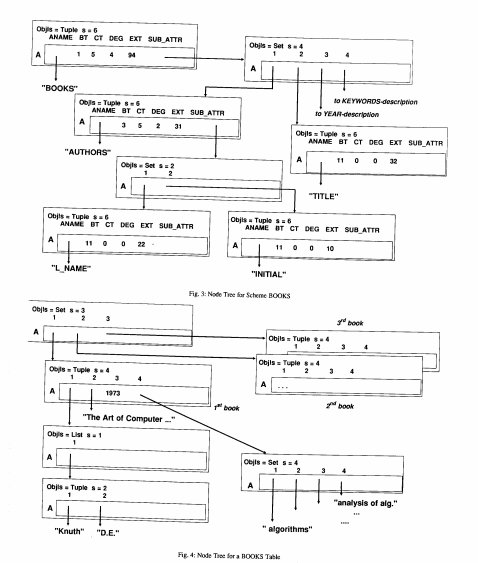
\includegraphics[scale=0.6]{Figures/VPDBEDIT.png}}
		\end{figure}

	\section{Libraries for Functionality}
		From GitHub Repositories, a list of Visual Scripting libraries are listed:-
		\begin{itemize}
		\item Language: GDScript - Author:~\href{https://github.com/swarnimarun}{Swarnimarun} - Respository:~\href{https://github.com/swarnimarun/visual-scripting-node-library}{Visual Scripting Node Library}.
		\item Language: Python - Author:~\href{https://github.com/leon-thomm}{leon-thomm} - Respository:~\href{https://github.com/leon-thomm/Ryven}{Ryven}.
		\item Language: C\# - Unity Game Engine - Author:~\href{https://github.com/ConstellationLanguage}{ConstellationLanguage} - Respository:~\href{https://github.com/ConstellationLanguage/Constellation}{Constellation}.
		\item Language: Web Scripting - Author:~\href{https://github.com/ericabouaf}{ericabouaf} - Respository:~\href{https://github.com/ericabouaf/webhookit}{webhookit}.
		\item Language: Web Scripting - Author:~\href{https://github.com/WebCabin}{WebCabin} - Respository:~\href{https://github.com/WebCabin/wcPlay}{wcPlay}.
		\end{itemize}

		These Visual Scripting software listed are identical to standard Game Engine Visual Scripting logic. Even though some are easy to use in the demos, a commonality is that they only allow users to control a live environment, whether it is a built-in game engine or an addition to an existing Game Engine, and they are mainly game oriented. VisualPro aims to support different platforms, such as Web, Mobile, Software, Data Analytics and Games. This aim is possible due to the diversity of users, adding new languages by entering the desired language within the XML document; though, it requires documentation to support users in adding new languages for the program to work correctly.

		A table of a few Web Builders and Visual Scripters demonstrates the difficulty of different platforms. Visual Scripting Software~\ref{tab:comp-1}:-
		\begin{table}[htbp]
			\caption{Comparison of Visual Scripters}
			\label{tab:comp-1}
			
			\resizebox{\columnwidth}{!}{%
			\begin{tabular}{cccc}
			\hline
			\textbf{Name}                               & \textbf{Description}                                                                                     & \textbf{Difficulty: Hard (0-10) Easy}                   & \textbf{Explanation?}                                                                                                                                                                                                                      \\ \hline
			\multicolumn{1}{c|}{Unreal Engine 5~\cite{unreal_engine_introduction_nodate}} & \multicolumn{1}{c|}{Game Engine (C++ Language)}                                                          & \multicolumn{1}{c|}{Beginner: 3-0 | Experience: 5-10}   & \begin{tabular}[c]{@{}c@{}}A beginner who does not \\ understand the principles of code \\ may struggle over time.\end{tabular}                                                                                                            \\ \hline
			\multicolumn{1}{c|}{Unity Engine~\cite{unity_technologies_unity_nodate}}    & \multicolumn{1}{c|}{Game Engine (C\# Language)}                                                          & \multicolumn{1}{c|}{Beginner: 2 - 6 | Experience: 8-10} & \begin{tabular}[c]{@{}c@{}}With the documentation available\\ and the simplicity of the Unity\\ Visual Scripting design, it seems\\ beginner-friendly.\end{tabular}                                                                        \\ \hline
			\multicolumn{1}{c|}{Minecraft~\cite{mojang_minecraft_nodate}}       & \multicolumn{1}{c|}{\begin{tabular}[c]{@{}c@{}}Game (Redstone)\\ Represents binary coding.\end{tabular}} & \multicolumn{1}{c|}{Beginner: 7-10 | Experience: 10}    & \begin{tabular}[c]{@{}c@{}}Even though Minecraft does not\\ create programming languages,\\ it shows that many ages who enjoy\\ logging onto Minecraft to make\\ Redstone functionality, passively\\ learn about Binary code.\end{tabular} \\ \hline
			\end{tabular}%
			}
			\end{table}

			After studying different Visual Scripting software, there is no portable Visual Scripting made for versatility. Both seem to only aim at Game Engines. Minecraft does not offer the ability for Visual Scripting. However, to bring attention to the Redstone feature in Minecraft, the feature is interesting for the audience, even to none-programmers. Could the VisualPro library be made into a Visual Scripting game, or specific in-game blueprints/prefabs be placed into the environment, generating code, so that the user can create programs whilst maintaining interest? Redstone accomplishes Binary teaching with Redstone passively by using on and off instead of 1s and 0s.

			Visual Scripting, Unreal Engine has a `messy' look, especially when the game logic is more clunky and complex, whereas Unity seems to have a better order. The problem with Visual Scripting in both engines is that the performance of the code is slow compared to writing the code manually. Would this uplift the software market sections if the VisualPro Scripting Pad software could generate code in the desired language with the most effective running time?

			\begin{table}[htbp]
			\centering
			\caption{Comparison of Web Builders}
			\label{tab:comp-2}
			\resizebox{\columnwidth}{!}{%
			\begin{tabular}{cccc}
			\hline
			\textbf{Name}                                                                   & \textbf{Description}             & \textbf{Difficulty: Hard (0-10) Easy}                  & \textbf{Explanation?}                                                                                                                                                                                                                  \\ \hline
			\multicolumn{1}{c|}{WordPress}                                                  & \multicolumn{1}{c|}{Web Builder} & \multicolumn{1}{c|}{Beginner: 8-10 | Experience: 9-10} & \begin{tabular}[c]{@{}c@{}}WordPress offers many\\ themes and plugins\\ to the user base.\end{tabular}                                                                                                                                 \\ \hline
			\multicolumn{1}{c|}{Wix}                                                        & \multicolumn{1}{c|}{Web Builder} & \multicolumn{1}{c|}{Beginner: 9-10 | Experience: 10}   & \begin{tabular}[c]{@{}c@{}}Wix is designed to help\\ buisnesses to design\\ webpages with no skill\\ required.\end{tabular}                                                                                                            \\ \hline
			\multicolumn{1}{c|}{\begin{tabular}[c]{@{}c@{}}Bootstrap\\ Studio\end{tabular}} & \multicolumn{1}{c|}{Web Builder} & \multicolumn{1}{c|}{Beginner: 5-7 | Experience: 7-10}  & \begin{tabular}[c]{@{}c@{}}Bootstrap Studio is a\\ similar interface to\\ Adobe Dreamweaver.\\ It offers templates and\\ allowed websites to designed.\\ This interface is difficult with\\ no experience with Bootstrap.\end{tabular} \\ \hline
			\end{tabular}%
			}
			\end{table}

			In one form, Web Builder's give an idea of what makes Visual Scripting easier. This concept is down to the research, design, and implementation of existing developers who had to look into individuals with no coding experience. If there is a correlation between designing a more straightforward Visual Scripting interface using methods that Web Builders introduced, it could update Visual Scripting and bring it into future software design. Perhaps, it could be a tool to visualise JavaScript so that users can build a website and add functionality, or create code snippets, for example, MelPy to animate 3D models within Autodesk Maya and other products, making Artists thrive more rather than relying on a Software Engineer to make their vision.

	\section{Testing Functionality}
		Testing functionality, whether performance, bugs or critical issues, is essential, especially before conducting any User Usability tests for many different reasons. The following scenario should create an understanding of why this stage is critical. 

		\begin{center}
			``Unit tests not only catch implementation bugs, but also have a positive effect on the design of the code under test (CUT) as they enforce testability [3]. Code developed without unit tests in place often has a much lower testability, which in turn increases the cost of retrofitting unit tests later on.'' - Clause Klammer~\cite{klammer_writing_2015}.
		\end{center}
		
		Trying to shape User Usability testing around Software with no unit testing creates a complex testability environment down the line. Clause Klammer's~\cite{klammer_writing_2015} states, `Code developed without unit tests in place often has a much lower testability...' that suggests further testing like Performance testing and User Usability tests could prove costly if poorly written code is in play. Furthermore, the Journal Article~\cite{klammer_writing_2015} argues that code is hard to maintain and proves more challenging to evolve, backed up by `As our experience taught us, the consequence is a heritage of legacy code that is hard to maintain and evolve.' Clause Klammer~\cite{klammer_writing_2015} raises the fact that after the implementation stage of the code, Unit Testing is rarely added and left alone, backed by `However, over years of working with legacy code, we found that unit tests are rarely added afterwards. Code that has not been developed in conjunction with unit tests right at the beginning typically remains without unit tests ever after which conforms to Don Well's statement: \textit{“If you do not start adding UnitTests today then one year from now you will still not have a good unit test suite.” [2]}'.
		
		Unit Testing is an excellent way of providing functionality testing, as a developer can create code directly from design plans before any implementation is committed or create and implement code around the test. From the Journal Article, Zenon Chaczko~\cite{chaczko_design_2014} suggests that unit testing indicates any flaws in the code and looks for any lousy programming practices. It is usually the case to pass a test before implementing the final product. Two unit tests are vital as the application uses both C\# .NET Framework 4.7.2 frontend and C++ backend. This process aids the software to meet a standard and provides the right results for both the developer and tester.
		
\chapter{Research Methodology}
\label{chap:researchMethodology}
	% \cite{hentati_fuzzy-logic_2016} - has information about how to set up the User Usability experiment
	This chapter describes the different methodologies available, methods of analysing the results and constructs an experiment that would provide insight on how User Usability should commence. After extensive research, four techniques closely reflect on VisualPro's testing. Quantitative Research, Qualitative Research, Descriptive Research, and Fundamental Research help justify the techniques VisualPro intends to help novice programmers.

	\textbf{Quantitative Research} enables calculations to provide answers to complex questions. This research method can measure productivity and User Usability to ensure the software is beginner-friendly. It is crucial to reflect on the calculations mentioned in the Literature Review to evaluate the data throughout the design period. \textbf{Qualitative Research} focuses on satisfaction experience, behaviours and intellect. A requirement of a complete analysis to check credibility. A survey inviting a mixed background of participants would support the research. \textbf{Descriptive Research} uses statistical data to analyse any design flaws within a project using official data. For accurate data that is relevant, the most up-to-date information dependent upon the scenario is suitable. \textbf{Fundamental Research} allows multiple research methods to correlate the information in a design plan. To justify the best research methodologies suitable for VisualPro's, Quantitative, Qualitative and Descriptive Research will support the design and development research of VisualPro. These methodologies help limit design flaws using up-to-date statistics, calculations to understand complications of comparing data to the gathered statistics, and any current design flaws within prototypes and VisualPro end implementation.

	The data collection requires a survey, screen recording and microphone data of applicants. This extra data will coincide with the Preference side of the test to understand if the software enables beginners to learn quickly with excellent UX and User Usability. 

	To gather feedback, a technique of two surveys, two tutorial documentation and video recordings of users using the application. The first survey is to collect feedback on how the design of the prototype, `Programming Planner', should feel if it had a UI applied to the software and suggestions of ways to improve the overall UX and User Usability of the software. This survey will prioritise \textit{Fundamental Research}, collecting both \textit{Qualitative} and \textit{Descriptive Research} to get as much detail as possible to make a Visual Scripting software that proves effective and easy to use in the novice section of the Software Engineering. An interesting point to make is that the `Don't Make Me Think, Revisited' book, authored by Steve Krug~\cite{krug_steve_dont_2014} suggests that `Testing one user is 100 percent better than testing none.' and `Testing one user early in the project is better than testing 50 near the end.' This suggestion is an ideal point to make as it suggests that early testing of the User Interface is a compelling idea to increase User Usability results during the creation period. To do this, the execution of the initial survey will test the prototype within a console application, using more experienced programmers, and then test the VisualPro User Interface within the final survey with both novice programmers and initial survey participants to ensure the User Interface is intuitive and easy to use.

	Two tutorials will give a temporary non-interactive learning environment to test the VisualPro in a learning environment for the second survey to work. Based on the research conducted, an interactive tutorial available inside VisualPro would help teach novice programmers by providing examples and other how-to exercises easier. However, having documented tutorials may benefit different learners who prefer a lightweight Visual Scripting pad without compulsory tutorial exercises and tips. Perhaps, a way to sort this problem is to provide a dialogue that asks the user three questions, `Skip All Learning Plans', `Interactive Learning' or `Non-Interactive Learning', changing the start-up procedure. Tutorial-A and Tutorial-B provide participants in the final survey with insight into how to write code in the VisualPro tool and teach basic OOP and FP styles.

	The second survey diverges into two sections, which are:-
	\begin{itemize}
		\item Programming Planner Improved vs VisualPro.
		\item Tutorial Questionnaire.
	\end{itemize}
	
	This survey aims to collect \textit{Descriptive Research} to gather research on whether VisualPro increases workflow compared to Programming Planner Improved and if VisualPro delivers a learning and valuable tool to novices when learning about Visual Scripting or Programming in general. The `Programming Planner Improved vs VisualPro' section is only applicable if the user has participated in the last survey. Within this section, the surveyee will answer a series of questions that reflect on their first answers to the first survey. Within the last section, all participants will observe and answer questions to test what they learned in the tutorial exercise and show their code generations. Results of whether the participant was successful, unclear or was unsuccessful are weighted, one being successful and zero being unsuccessful. If any generated code is on the right lines, they have a value of 1. If any input code is unclear, as in the copied code has any errors but the answers to the exercise questions are fitting, they have a value of 0.5. Otherwise, they are assigned the value of 0.

	% Video footage
	The final survey asks participants for video footage containing screen recordings using VisualPro Visual Scripting software; no requirement for the video or audio content. The footage provides an analytic opportunity to test if the software provides excellent UX and User Usability for novice and experienced programmers. This approach delivers Descriptive Research to encourage a comprehensive analysis of the UX and User Usability to enhance the quality of VisualPro's UI before forming the product further.

	% Result number likings (each one)
	Examining the `Don't Make Me Think, Revisited' book, authored by Steve Krug~\cite{krug_steve_dont_2014} justifies what type of results are a reasonable aim for collecting research. In the chapter "Chapter 9. Usability testing on 10 cents a day", the author highlights that '...Focus groups are not usability tests.' indicating that whilst gathering information on whether the participants could generate code with little knowledge, it does not make it an easy-to-use and idealistic UX and User Usability. To back this up, following a tutorial could stimulate more promising results than trying the software with no expert guide. Hence, gathering video content of the participant following the tutorial will help examine the User Usability to see their initial intentions.
	
	Further within the chapter, a few points including:-
	\begin{center}
		``Here's the difference in a nutshell:
		\begin{itemize}
			\item In a \textbf{focus group}, a small group of people (usually 5 to 10) sit around a table and talk about things, like their opinions about products, their past experiences with them, or their reactions to new concepts. Focus groups are good for quickly getting a sampling of users` feelings and opinions about things.
			\item \textbf{Usability} tests are about watching one person at a time try to use something\\(whether it`s a Web site, a prototype, or some sketches of a new design) to do typical tasks so you can detect and fix the things that confuse or frustrate them.
		\end{itemize}
		'' - Steve Krug~\cite{krug_steve_dont_2014}.
	\end{center}

	Ranging from the suggestion of five to ten respondents, an audience of six surveyees is ample for the survey. Two of these respondents will have done the initial survey to gather data to compare Programming Planner to VisualPro. As the video research is optional, two to three video demonstrations are within the expectations. However, as the survey focuses on the results of VisualPro code generation, both can provide good UX and User Usability results.

	`Measuring Usability: Preference vs. Performance', written by Jakob Nielsen and Jonathon Levy~\cite{nielsen_measuring_1994} experiments to determine whether Preference and Performance influenced each other. The VisualPro results could indicate a clear correlation if the theory stands true.
	Unfortunately, the authors could not conclude whether they did or not. This analysis aims to determine methods to create a Visual Scripting language that helps novices' with little-to-none experience whilst increasing the overall performance of computing projects. Video content of users' using the VisualPro software provides insight into how the user navigates the software and whether they try any features that are non-existent that show preferences that could lead to feature ideas. A Fuzzy Expert Logic system can help decipher whether the user was using the software effectively.

	% Evaluate Data with Fuzzy Logic %
	Fuzzy Expert logic will help identify the performance level of a User Usability category by three following categories, `Hard Usability', `Moderate Usability' and `Easy Usability'. A conversion of the performance results from the final study using the Fuzzy Expert logic to identify the three categories. The same application of the previous method helps convert the preference results from the initial research. The following information could help indicate whether performance and preference contradict each other and may help determine if the initial study did help create a better UX and User Usability result.

	% Performance Fuzzy Expert Logic %
	% 100% / 3
	\textbf{Performance Fuzzy Logic Setup:-}
	\begin{center}
		\textbf{Mathematical Key: }\\
		$\mathcal{U}$ = Usability Categories: `Hard Usability', `Moderate Usability' and `Easy Usability'.\\
		$\mathcal{P}$ = Performance Categories: `Very Low', `Low', `High' and `Very High'.\\
		$\mathcal{VL}$ = Performance Category: `Very Low (0\%)'. - $\mathcal{L}$ = `Low (25\%).'\\
		$\mathcal{H}$ = Performance Category: `High (75\%)'. - $\mathcal{VH}$ = `Very High (100\%)'.\\
		$\mathcal{R}$ = Responses with Performance Categories. - $\mathcal{T}$ = An array of responses.\\

		\[\mathcal{U} = \sum_{n = 0}^{3} \frac{100}{3} - (n = n + 5) \rightarrow \left|
			\begin{array}{ccc}
				\mathcal{HU} & \mathcal{MU} & \mathcal{EU}
			\end{array} \right|
		\]
		\[\mathcal{P} = \frac{100}{4} \rightarrow \left|
			\begin{array}{cccc}
				\mathcal{VL} & \mathcal{L} & \mathcal{H} & \mathcal{VH}
			\end{array} \right|
		\]
		\[ \mathcal{R}_{P} = \left| 
			\begin{array}{c}
				T_{n}
			\end{array}
		 \right|
		\]

		$\sum_{n = 1}^{n < R_{n}} \mathcal{M_{n}} = \frac{R_{i}}{R_{T}}$
	\end{center}
		
	% Mathematical Sign %
	Essentially to work out the Performance figures, calculation of the code submissions within the survey to generate a percentage. Four statements measured by $\mathcal{P}$, `The respondent followed the task correctly', `The respondent seems to have followed the task correctly', `The respondent seems to have followed the task incorrectly' and `The respondent followed the task incorrectly' helps to determine the performance level. Each respondent's results are tallied up and positioned in the $\mathcal{R_{P}}$ array, which provides a performance level of each respondent. Sum of $\mathcal{P}$ of each $\mathcal{R}$ element and then divided by the $\mathcal{T_{n}}$ provides an average percentage. The $\mathcal{U}$ identifies the Fuzzy Expert categories percentage with added weights. The weighing strategy should enable the analysis to be unbiased.

	% Mathematical Sign %
	From the initial survey, a selection of two preference questions including Figure~\ref{fig:q-11} - `According to you, how should the features of the Graphical User Interface have to work?' and Figure~\ref{fig:q-12} - `How would you prefer to access the software?' helps work out the preference level. A calculation to sort out each categories with the responses and whether or not the preference is within the VisualPro design implementation. To filter the preference down, only the preferences within the VisualPro design implementation are taken into account. The mean of the preference of each category is then calculated and then inserted into the Fuzzy Expert logic. The preference and performance levels are then compared to determine the overall User Usability and analyse whether preference affects performance.
	
\chapter{Prototype}
\label{chap:prototype}
	To access the prototype that demonstrates communication from a .NET Framework 4.7.2 to a C++ backend library, go to~\href{https://github.com/ShinkuKira21/VisualPro-FinalProject/tree/main/Prototypes/GUI%20Concept%20.NET-C%2B%2B/Package}{Prototypes/GUI Prototype .NET-C++}~\cite{patch_visualpro_2022}. Even though this prototype is not related to the current project, it demonstrates how the frontend can interact with the backend and provides insight into how this is possible. The purpose of the application is not to measure the application's performance merely to provide insight and experience on how the application communicates to the backend.

	The source code, found in~\href{https://github.com/ShinkuKira21/VisualPro-FinalProject/tree/main/Prototypes/GUI%20Concept%20.NET-C%2B%2B/Source%20Code}{Prototypes/GUI Prototype .NET-C++}~\cite{patch_visualpro_2022}, demonstrates the functionality to load the DLLs within the application. Implementation of two techniques follows:-
	\begin{itemize}
		\item \textit{DllImportAttribute} (Enables the ability to import Native DLLs into the application).
		\item \textit{\_declspec(dllexport)} (C communication files use this to create entry points.)
	\end{itemize}

	\begin{figure}[H]
		\ffigbox[\FBwidth] {
			\caption[GUI Prototype]{GUI Prototype Communication C\# to C++}
			\label{fig:guiPrototype}
		}
		{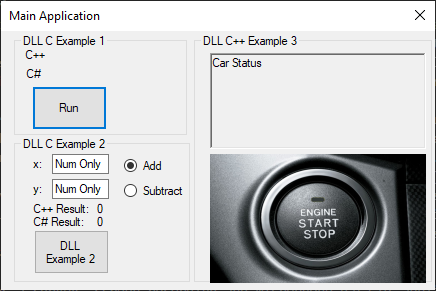
\includegraphics[scale=1]{Figures/applications/prototype.png}}
	\end{figure}

\chapter{Design and Feedback}
\label{chap:designAndFeedback}
	The Design and Feedback section covers the Research Methodology and the Pre-Planning, which shows the steps and the level of thought that went into deciding VisualPro's purpose and the existing software and prototypes. Some Notebook Planning may not make sense as some foreseeable problems were thought and planned ahead of time.
	
	\section{Pre-Planning}
		\subsection{HTML Design} 
			Figure~\ref{fig:htmlDesign} shows a HyperText Markup Language (HTML) Design of how the UI should look. The Empty Column is where the user drops elements like Classes, Functions or Variables. Buttons on the right can be dragged and dropped on the Empty Column to the left. The functionality of the drop should create a new container, giving the user acknowledgement there's a new parent or sub-element with room for configuration and another drag and drop container within the class or function.

			\begin{figure}[H]
				\ffigbox[\FBwidth] {
				\caption[UI Illustration]{HTML Design - Found at: \href{https://github.com/ShinkuKira21/VisualPro-FinalProject/blob/main/Showcase-Work_Completed/PrePlanning\%20(Whole\%20Idea)/HTML_Design.jpg}{Original Image}}
				\label{fig:htmlDesign}
				}
				{\includegraphics[scale=0.55]{{"../../Showcase-Work_Completed/PrePlanning (Whole Idea)/HTML_Design"}.jpg}}
			\end{figure}

		\subsection{Notebook Page 1-2} 
			Figure~\ref{fig:nb-1} contains numerous ideas. Page 1 contains a heading, 'Personal Assistant', which indicates the thought process of a personal assistant before the Visual Programming Scripting program progressed. After planning this, it became apparent to use a type of Artificial Intelligence (AI), which knew the basic syntax of different languages and would write or advise the user when typing. This process is very similar to TabNine~\cite{noauthor_code_nodate}.

			The second page of this figure, shows a few different examples of IF statement syntax from lafnguages to find a `dynamic' common rather than keep it static like the previous software. The sketch below shows a name for the software and a example of how the language selection would look on UI.

			\begin{figure}[H]
				\ffigbox[\FBwidth] {
				\caption[Notebook P-1.2]{Notebook Plan Page 1-2 - Found at: \href{https://github.com/ShinkuKira21/VisualPro-FinalProject/blob/main/Showcase-Work_Completed/PrePlanning\%20(Whole\%20Idea)/NP1.jpg}{Original Image}}
				\label{fig:nb-1}
				}
				{\includegraphics[scale=0.45]{{"../../Showcase-Work_Completed/PrePlanning (Whole Idea)/NP1"}.jpg}}
			\end{figure}
			
		\subsection{Notebook Page 2-3} 
			Figure~\ref{fig:nb-2} displays two pages of how the Visual Scripting could look. The top page shows the tools on the left, such as Logical, Structure and Scoping tools. On the right, it should show a list of current variables, functions and classes in a hierarchy style. The middle of the application is the work area.
			\begin{figure}[H]
				\ffigbox[\FBwidth] {
				\caption[Notebook P-3.4]{Notebook Plan Page 3-4 - Found at: \href{https://github.com/ShinkuKira21/VisualPro-FinalProject/blob/main/Showcase-Work_Completed/PrePlanning\%20(Whole\%20Idea)/NP2.jpg}{Original Image}}
				\label{fig:nb-2}
				}
				{\includegraphics[scale=0.6]{{"../../Showcase-Work_Completed/PrePlanning (Whole Idea)/NP2"}.jpg}}
			\end{figure}

		\subsection{Notebook Page 5-6} 
			Figure~\ref{fig:nb-3} gives the planning of how the syntax for most programming and scripting languages. The plan points out patterns and tries to identify their names for the Extensible Markup Language (XML) and backend to comprehend. This piece of planning helped excel the development of the program's dynamic side to allow the addition of new languages to the software.
			\begin{figure}[H]
				\ffigbox[\FBwidth] {
				\caption[Notebook P-5.6]{Notebook Plan Page 5-6 - Found at: \href{https://github.com/ShinkuKira21/VisualPro-FinalProject/blob/main/Showcase-Work_Completed/PrePlanning\%20(Whole\%20Idea)/NP3.jpg}{Original Image}}
				\label{fig:nb-3}
				}
				{\includegraphics[scale=0.45]{{"../../Showcase-Work_Completed/PrePlanning (Whole Idea)/NP3"}.jpg}}
			\end{figure}

		\subsection{Notebook Page 7-8} 
			Figure~\ref{fig:nb-4} demonstrates how the XML would possibly look. The table shows N (Node), A (Attribute) and the Meaning. To explain what is going on, Node |0| is the header node (holds library data such as \textbf{system} or \textbf{iostream}), holds three attributes. Attribute |0| holds `Type', which is the purpose, Attribute |1| holds the `Name', which is the library's name. Attribute |2| holds the `Syntax Value', which in C\# it is \textit{using ;} and in C++, the value is \textit{\#include $<>$} .
	
			According to the second node |1| holds information for structure or classes in languages. This node contains three attributes. Attribute |0| holds `Name of Struct \textit{(or)} Class', which contains the user-defined name they have created inside VisualPro. Attribute |2| holds the `Properties' like the member of the struct/class. Attribute |3| holds the syntax value, the open and close case of a struct/class and layout within the struct/class.
	
			\begin{figure}[H]
				\ffigbox[\FBwidth] {
				\caption[Notebook P-7.8]{Notebook Plan Page 7-8 - Found at: \href{https://github.com/ShinkuKira21/VisualPro-FinalProject/blob/main/Showcase-Work_Completed/PrePlanning\%20(Whole\%20Idea)/NP4.jpg}{Original Image}}
				\label{fig:nb-4}
				}
				{\includegraphics[scale=0.45]{{"../../Showcase-Work_Completed/PrePlanning (Whole Idea)/NP4"}.jpg}}
			\end{figure}
	
		\subsection{Notebook Page 9-10}
			Figure~\ref{fig:nb-5} answers how the loops and logical statements work in the LanguageCompiler library. This planning shows how the XML nodes and the Planner List should work together. In theory, the Planner List, of what the user populates with the program's use, combines with the XML document with the chosen language.

			\begin{figure}[H]
				\ffigbox[\FBwidth] {
				\caption[Notebook P-9.10]{Notebook Plan Page 9-10 - Found at: \href{https://github.com/ShinkuKira21/VisualPro-FinalProject/blob/main/Showcase-Work_Completed/PrePlanning\%20(Whole\%20Idea)/NP5.jpg}{Original Image}}
				\label{fig:nb-5}
				}
				{\includegraphics[scale=0.45]{{"../../Showcase-Work_Completed/PrePlanning (Whole Idea)/NP5"}.jpg}}
			\end{figure}
	
		\subsection{Notebook Page 11} 
			Figure~\ref{fig:nb-6} displays how the function node should work. This miniature theory is to help the developer understand how the XML document should work in a progr ammatical sense. This again helped when it comes to the prototypes further in this document.
	
			\begin{figure}[H]
				\ffigbox[\FBwidth] {
				\caption[Notebook P-11]{Notebook Plan Page 11 - Found at: \href{https://github.com/ShinkuKira21/VisualPro-FinalProject/blob/main/Showcase-Work_Completed/PrePlanning\%20(Whole\%20Idea)/NP6.jpg}{Original Image}}
				\label{fig:nb-6}
				}
				{\includegraphics[scale=1]{{"../../Showcase-Work_Completed/PrePlanning (Whole Idea)/NP6"}.jpg}}
			\end{figure}
	
		%recheck-$41%
		\newpage
		\subsection{Notebook Page 12-13} 
			Figure~\ref{fig:nb-7} shows a predicted problem is as follows:
			\begin{center}
				\textbf{Description:}\\ How will the program know where to put a sub-child and how will it?
			
				\textbf{Answer:}\\ The planner would hold its parent and sub identity, and the Triangle (30 Code) symbol tells the software where to put the child. The Triangle symbol will only appear of classes or functions that have children. This means that the program will focus on parents, close the tags, then rescan to put the children in the code. The problem before is that it would be hard to tell the program to remember when and where to close tags if it got too deep in theory.
			\end{center}
	
			\begin{figure}[H]
				\ffigbox[\FBwidth] {
				\caption[Notebook P-12.13]{Notebook Plan Page 12-13 - Found at: \href{https://github.com/ShinkuKira21/VisualPro-FinalProject/blob/main/Showcase-Work_Completed/PrePlanning\%20(Whole\%20Idea)/NP7.jpg}{Original Image}}
				\label{fig:nb-7}
				}
				{\includegraphics[scale=0.45]{{"../../Showcase-Work_Completed/PrePlanning (Whole Idea)/NP7"}.jpg}}
			\end{figure}
	
		%recheck-$41%
		\newpage
		\section{Results of Feedback}
			\subsection{Survey Question 1}
			\label{subsec:rof-sq1}
				According to the chart~\ref{fig:q-1}, \textit{87.5\%} chose `Programming Planner Improved', and \textit{12.5\%} chose `None of the Above' to the question, `As a developer, which program worked for you?'. This data suggests that most of the responses preferred `Programming Planner Improved' out of eight. The response may suggest that participants enjoyed the interface as it offers more than the Programming Planner. However, the \textit{12.5\%} of the `None of the Above' option displays that the application may prove tedious for some.
				\begin{figure}[H]
					\ffigbox[\FBwidth] {
					\caption[Survey Q-1]{Survey Question 1 - Found at: \href{https://github.com/ShinkuKira21/VisualPro-FinalProject/blob/main/Showcase-Work_Completed/Surveying/q1.png}{Original Image}}
					\label{fig:q-1}
					}
					{\includegraphics[scale=0.50]{{"../../Showcase-Work_Completed/Surveying/q1"}.png}}
				\end{figure}

			\subsection{Survey Question 2}
				Figure~\ref{fig:q-2} asks the question, `If the last option on the previous question is ticked, then explain why?'. Four responses replied with:-
				\begin{itemize}
					\item `More flexibility' -\\
							This response could mean two things: the Programming Planner Improved is more flexible than the first program or that both programs would benefit from more flexibility.
					\item `Both work' -\\
							This response indicates that both software works.
					\item `The option to choose the desired programming language at the end of the programming' -
							A surveyee liked the option in Programming Planner Improved to select different programming languages.
					\item `Because it had more options and had example code at the end of planning' -
							This answer describes that the Programming Planner Improved offered more options, such as argument selection and code language.
				\end{itemize}
		
				\begin{figure}[H]
					\ffigbox[\FBwidth] {
					\caption[Survey Q-2]{Survey Question 2 - Found at: \href{https://github.com/ShinkuKira21/VisualPro-FinalProject/blob/main/Showcase-Work_Completed/Surveying/q2.png}{Original Image}}
					\label{fig:q-2}
					}
					{\includegraphics[scale=0.45]{{"../../Showcase-Work_Completed/Surveying/q2"}.png}}
				\end{figure}
		
			\subsection{Survey Question 3} 
				Figure~\ref{fig:q-3} asks the question to Surveyee's, `Did the tutorial at the beginning of Programming Planner Improved help navigate around the application?'. This question tries to find out if the application is hard to use overall. The responses were 87.5\% for yes, and 12.5\% for no. Even though the most of the responses chose yes, the application may still be hard to use if, theoretically, one out of eight users found the UX frustrating or confusing.

				\begin{figure}[H]
					\ffigbox[\FBwidth] {
					\caption[Survey Q-3]{Survey Question 3 - Found at: \href{https://github.com/ShinkuKira21/VisualPro-FinalProject/blob/main/Showcase-Work_Completed/Surveying/q3.png}{Original Image}}
					\label{fig:q-3}
					}
					{\includegraphics[scale=0.45]{{"../../Showcase-Work_Completed/Surveying/q3"}.png}}
				\end{figure}
		
			\subsection{Survey Question 4}
				Figure~\ref{fig:q-4}, `What makes the Programming Planner Improved better than the previous product?' checkbox question, offered five qualities. These are:-
				\begin{itemize}
					\item \textbf{Ease of Use} - Aimed to find out how easy the application is easy to use. 50\% of the responses think it was easier to use than the previous product. This feedback could mean to things, the first product was similar and consequently did not improve the application in this quality or that the product needs to improve in this area.
					\item \textbf{Performance} - To see if the audience could notice any performance difference. This quality is vital as a Graphical User Interface (GUI) can somewhat be `chunky'. The responses were 0\% out of the responses; though this may seem negative, it is sometimes hard to notice the difference between console and desktop applications.
					\item \textbf{Extra Features} - The quality, `Extra Features`, displays if the extra features in the new application stood out and improved the previous application. The responses were 62.5\%, which indicates that the extra features did stand out and made the application better.
					\item \textbf{File Structure} - The quality, `File Structure' of the second application is revised and stores the saved file in a directory other than the ROOT directory. 25\% of the responses chose this option, which means that the File Structure did not impact the application as effectively as the `Extra Features' quality.
				\end{itemize}

				\begin{figure}[H]
					\ffigbox[\FBwidth] {
					\caption[Survey Q-4]{Survey Question 4 - Found at: \href{https://github.com/ShinkuKira21/VisualPro-FinalProject/blob/main/Showcase-Work_Completed/Surveying/q4.png}{Original Image}}
					\label{fig:q-4}
					}
					{\includegraphics[scale=0.45]{{"../../Showcase-Work_Completed/Surveying/q4"}.png}}
				\end{figure}
		
			\subsection{Survey Question 5}
				Figure~\ref{fig:q-5} asks the Surveyee's, `Explain your answer' to the last question. This question will tell what the Surveyee's felt when answering the last question. The responses are as follows:
				\begin{itemize}
					\item `More features allowed for a wider range of approaches' - This specific feedback suggests that it is better to add more functionality in the GUI application to allow for more usability.
					\item `More languages and was easier to use. Very impressed' - This response implies that the idea of a dynamic language interface to allow users to add more languages will increase User Experience.
					\item `Easier to use, the better' - Visual Scripting already is complicated when looking at the Unreal Engine's Visual Scripting interface. If it is possible to create a lightweight Visual Scripting pad to allow a programmer to create code snippets, it could bring more developers into the field and increase production time already in the field.
					\item `Have not used the previous version' - This suggests that the Surveyee only tested Programming Planner Improved.
					\item `Allowed me to create a function structure and save it. Seemed difficult to follow (variables weren' numbered)' - According to this response, the user found it difficult to follow through and should be something to think about when making the GUI application.
					\item `Easy, helpful and understandable' - This response shows that the user found the software easy to use, helpful and understanding during their experience.
					\item `The extra features added to the improved version of the program improve used experience by adding expanded usability' - The response suggests that again the extra functionality helped improve the User Experience, in Programmer Planner Improved.
					\item `It just had extra features and seemed more useful' - Which implies that the user found the extra features more comfortable and useful to use.
				\end{itemize}
		
				\begin{figure}[H]
					\ffigbox[\FBwidth] {
					\caption[Survey Q-5]{Survey Question 5 - Found at: \href{https://github.com/ShinkuKira21/VisualPro-FinalProject/blob/main/Showcase-Work_Completed/Surveying/q5.png}{Original Image}}
					\label{fig:q-5}
					}
					{\includegraphics[scale=0.45]{{"../../Showcase-Work_Completed/Surveying/q5"}.png}}
				\end{figure}
		
			\subsection{Survey Question 6}
			\label{subsec:rof-sq6}
				Figure~\ref{fig:q-6} asks the Surveyee, `How would you rate the User Experience (overall)?'. The question tries to aim for an idea of how the UX of the two products. On a scale of one (Stressful) to ten (Relaxing), 62.5\% of the responses went with option eight, 37.5\% of the responses went with option seven. These figures show that the UX has room for improvement. When designing and implementing the GUI product, it is important to think about the UI and UX.

				\begin{figure}[H]
					\ffigbox[\FBwidth] {
					\caption[Survey Q-6]{Survey Question 6 - Found at: \href{https://github.com/ShinkuKira21/VisualPro-FinalProject/blob/main/Showcase-Work_Completed/Surveying/q6.png}{Original Image}}
					\label{fig:q-6}
					}
					{\includegraphics[scale=0.45]{{"../../Showcase-Work_Completed/Surveying/q6"}.png}}
				\end{figure}
				
			\subsection{Survey Question 7}
				Figure~\ref{fig:q-7} asks the question, `How useful is Programming Planner for beginners?'. This question is done on a scale of one (Complicated) to five (Useful). The feedback is ranged from one to five and suggests that beginners may find this platform hard work. The responses are as follows:
				\begin{itemize}
					\item \textbf{One} - 25\% responses. These respondents reckon that Programming Planner is complicated for beginners.
					\item \textbf{Three} - 12.5\% responses. These respondents thought that Programming Planner is a little complicated for beginners.
					\item \textbf{Five} - 50\% responses. These respondents figure that Programming Planner is close to Useful for beginners.
					\item \textbf{Six} - 12.5\% responses. These respondents consider that Programming Planner is Useful for beginners. 
				\end{itemize}
		
				\begin{figure}[H]
					\ffigbox[\FBwidth] {
					\caption[Survey Q-7]{Survey Question 7 - Found at: \href{https://github.com/ShinkuKira21/VisualPro-FinalProject/blob/main/Showcase-Work_Completed/Surveying/q7.png}{Original Image}}
					\label{fig:q-7}
					}
					{\includegraphics[scale=0.45]{{"../../Showcase-Work_Completed/Surveying/q7"}.png}}
				\end{figure}
				
			\subsection{Survey Question 8}
			\label{subsec:rof-sq8}
				Question~\ref{fig:q-8} `Did this help create a structure of your favourite language faster than standard methods?'. 75\% of responses said Yes, 12.5\% of responses said `Would not recommend to new programmer as they will not learn the basics' and 12.5\% said `I have not used other methods'. This chart suggests that the majority found this software to be faster than their standard methods.
				\begin{figure}[h]
					\centering
					\includegraphics[width=0.85\columnwidth]{{"../../Showcase-Work_Completed/Surveying/q8"}.png}
					\caption{Survey Question 8 - Found at: \href{https://github.com/ShinkuKira21/VisualPro-FinalProject/blob/main/Showcase-Work_Completed/Surveying/q8.png}{Original Image}}
					\label{fig:q-8}
				\end{figure}
		
			\subsection{Survey Question 9}
				Question~\ref{fig:q-9} `What features would you wish Programming Planner to offer?'. This question attempts to determine if the user has any requests about the software they have used. These were the responses:-
				\begin{itemize}
					\item `When I wanted only one function on the variable creation it asked if it works with other functions but I didn't have any other functions' - This suggestion shows that the user was confused with the way the program asked the user if the variable was a argument or a standard variable.
					\item `The target audience for this program will have little coding experience, and may forget what is required of a function, variable, etc. Adding examples to each page may be a good idea to reduce confusing.' - This suggestion shows that a help page or tips pop up on creating an element within the GUI program will help beginners use this software.
					\item `A set of pre made open source programs that could be quickly accessed' - Perhaps, the program could offer a GitHub repository import, which will examine the code and visualise it for the user.
					\item `Would be better with visualisation if writing a longer program' - The response could mean two things. It could mean that the user wanted to have an ability to overview the code within the console application, or it could mean that the user would have preferred a GUI work area.
					\item `A GUI' - This response means that the user would have preferred a GUI product rather than a console application.
					\item `Allow sudo code comments to be added to the function' - In the GUI application, it could have the ability for the user to enter comments.
					\item `Calculator?' - This response did not seem useful to add in to the future software, as popup calculators are available in most operating systems.
				\end{itemize}
		
				\begin{figure}[H]
					\ffigbox[\FBwidth] {
					\caption[Survey Q-9]{Survey Question 9 - Found at: \href{https://github.com/ShinkuKira21/VisualPro-FinalProject/blob/main/Showcase-Work_Completed/Surveying/q9.png}{Original Image}}
					\label{fig:q-9}
					}
					{\includegraphics[scale=0.45]{{"../../Showcase-Work_Completed/Surveying/q9"}.png}}
				\end{figure}
		
			\subsection{Survey Question 10}
			\label{subsec:rof-sq10}
				Figure~\ref{fig:q-10} ask `Would a Graphical User Interface uplift the User Experience?' as a multiple-choice question. The 100\% chose the yes choice. This feedback implies that they would like a GUI to work with over a console application out of the eight responses.
				\begin{figure}[H]
					\ffigbox[\FBwidth] {
					\caption[Survey Q-11]{Survey Question 10 - Found at: \href{https://github.com/ShinkuKira21/VisualPro-FinalProject/blob/main/Showcase-Work_Completed/Surveying/q10.png}{Original Image}}
					\label{fig:q-10}
					}
					{\includegraphics[scale=0.45]{{"../../Showcase-Work_Completed/Surveying/q10"}.png}}
				\end{figure}
		
			\subsection{Survey Question 11} 
				A grid question asked `According to you, how should the features of the Graphical User Interface have to work?'. The following options are: `Clickable', `Drag and Drop', `Drop Down Menu' and `Text Filled'. The details are `Structure Elements', `Logic Elements', `Select Languages and Save' and `Sub Elements'. After overlooking the table~\ref{fig:q-11} `Structure Elements' looks like it favoured Drag and Drop the most by four responses. The Drag and Drop were also voted for the `Logic Elements' by five responses. The `Select Languages and Save' preferred the Drop Down Menu by six responses, and lastly, the `Sub Elements' liked the idea if it was Text Filled.

				\begin{figure}[H]
					\ffigbox[\FBwidth] {
					\caption[Survey Q-11]{Survey Question 11 - Found at: \href{https://github.com/ShinkuKira21/VisualPro-FinalProject/blob/main/Showcase-Work_Completed/Surveying/q11.png}{Original Image}}
					\label{fig:q-11}
					}
					{\includegraphics[scale=0.45]{{"../../Showcase-Work_Completed/Surveying/q11"}.png}}
				\end{figure}
		
			\subsection{Survey Question 12} 
				This grid asks the participants, `How would you prefer to access the software?'. The options are `Windows Operating System', `Linux Operating System', `ChromeOS/Android' and `iOS'. The details are `Computer, Laptop or Tablet Devices', `Web Application', `Mobile Devices'. For the first column, the responses favour the Windows Operating System by eight. The second column, Windows Operating System, is also preferred by eight. The last column, ChromeOS, is the six responses favourites, and iOS is preferred by four. After reviewing this, the application aims for the Windows Operating System to get the most attention. Programming Planner and Programming Planner Improved works for both Windows and Linux Operating Systems.
				\begin{figure}[H]
					\ffigbox[\FBwidth] {
					\caption[Survey Q-12]{Survey Question 12 - Found at: \href{https://github.com/ShinkuKira21/VisualPro-FinalProject/blob/main/Showcase-Work_Completed/Surveying/q12.png}{Original Image}}
					\label{fig:q-12}
					}
					{\includegraphics[scale=0.45]{{"../../Showcase-Work_Completed/Surveying/q12"}.png}}
				\end{figure}
		
			\subsection{Survey Question 13}
				Figure~\ref{fig:q-13} a question, `Any comment?' follows the last questions. The only response was `No'.

				\begin{figure}[H]
					\ffigbox[\FBwidth] {
					\caption[Survey Q-13]{Survey Question 13 - Found at: \href{https://github.com/ShinkuKira21/VisualPro-FinalProject/blob/main/Showcase-Work_Completed/Surveying/q13.png}{Original Image}}
					\label{fig:q-13}
					}
					{\includegraphics[scale=0.45]{{"../../Showcase-Work_Completed/Surveying/q13"}.png}}
				\end{figure}
		
			\subsection{Survey Question 14-15}
				Figures~\ref{fig:q-14} and~\ref{fig:q-15} shows two questions, `How complicated is Visual Scripting? (Reference to Unreal Engine for an example).' Furthermore, `How complicated is Website Builders?' these questions portray how existing Visual Scripting Web Builders are successful, and if it is possible to do a service that is easier to use, similar to a web builder. The question is on a scale of one (Piece of Cake) to five (Complicated). The feedback from the first question:-
				\begin{itemize}
					\item Three - 37.5\% of the responses. This indicates that this percentage of the participants find Visual Scripting moderately easy.
					\item Four - 50\% of the responses. This displays that 50\% of the participants find Visual Scripting a bit more complicated than the 37.5\%.
					\item Five - 12.5\% of the responses find Visual Scripting tough.
				\end{itemize}
		
				The feedback from the second question:-
				\begin{itemize}
					\item One - 25\% of the responses find Web Builders a `Piece of Cake'.
					\item Two - 50\% of the responses find Web Builders more or less easy.
					\item Three - 25\% of the responses find Web Builders moderately easy.
				\end{itemize}
		
				These findings will change the research perspective to look more into the Web Builder layouts, functionality and UX to work out the GUI of the product.
		
				\begin{figure}[H]
					\ffigbox[\FBwidth] {
					\caption[Survey Q-14]{Survey Question 14 - Found at: \href{https://github.com/ShinkuKira21/VisualPro-FinalProject/blob/main/Showcase-Work_Completed/Surveying/q14.png}{Original Image}}
					\label{fig:q-14}
					}
					{\includegraphics[scale=0.45]{{"../../Showcase-Work_Completed/Surveying/q14"}.png}}
				\end{figure}

				\begin{figure}[H]
					\ffigbox[\FBwidth] {
					\caption[Survey Q-15]{Survey Question 15 - Found at: \href{https://github.com/ShinkuKira21/VisualPro-FinalProject/blob/main/Showcase-Work_Completed/Surveying/q15.png}{Original Image}}
					\label{fig:q-15}
					}
					{\includegraphics[scale=0.45]{{"../../Showcase-Work_Completed/Surveying/q15"}.png}}
				\end{figure}
		
			\subsection{Survey Question 16}
				Question~\ref{fig:q-16}, `If Programming Planner had an easy-to-use drag and drop feature without input and output relationships, then will this improve Visual Scripting overall?', the question paints a picture from the participants to see if the relationships in Visual Scripting that is similar to Entity-Relationship Diagrams if they cause a problem. All eight responses replied back with yes.

				\begin{figure}[H]
					\ffigbox[\FBwidth] {
					\caption[Survey Q-16]{Survey Question 16 - Found at: \href{https://github.com/ShinkuKira21/VisualPro-FinalProject/blob/main/Showcase-Work_Completed/Surveying/q16.png}{Original Image}}
					\label{fig:q-16}
					}
					{\includegraphics[scale=0.45]{{"../../Showcase-Work_Completed/Surveying/q16"}.png}}
				\end{figure}
		
			\subsection{Survey Question 17}
				Similar to the previous question to paint an image from what the participants want to see, `Would Visual Scripting be better if it allowed users to add any language they wish and generate any language with one click of a button?'. According to the figure~\ref{fig:q-17}, all of the eight responses responded with yes.

				\begin{figure}[H]
					\ffigbox[\FBwidth] {
					\caption[Survey Q-17]{Survey Question 17 - Found at: \href{https://github.com/ShinkuKira21/VisualPro-FinalProject/blob/main/Showcase-Work_Completed/Surveying/q17.png}{Original Image}}
					\label{fig:q-17}
					}
					{\includegraphics[scale=0.45]{{"../../Showcase-Work_Completed/Surveying/q17"}.png}}
				\end{figure}
		
			\subsection{Survey Question 18} 
				To squeeze more information from the participants, a question, `What was the reason for your selection?' was asked and made compulsory. The responses are as follows:-
				\begin{itemize}
					\item `Would be easier to write programs (for some people)'
					\item `A feature such as this would greatly reduce the production times involved in program development.'
					\item `save time and allow users to focus on the details'
					\item `I would like to code in any language I choose if that option was applicable.'
					\item `Useful feature'
					\item `Makes it more visual'
					\item `Again, the easier to use, and the more features, the better'
					\item `More accessibility'
				\end{itemize}
		
				After reading the feedback, a few points are to address. The current software already makes it easier to write code for some people, so it is imperative that the new software does not distract but improve the capability of writing software. The command-line may benefit users as it keeps developers in a similar environment they are probably already using. Another point to address is this question, `Will the GUI software get too heavy with too many features making it no longer lightweight?'. The best thing about having Dynamic-Link Libraries is that developers can incorporate into Java Android, iOS, Web Applications and, but not limited to, Visual Studio Code Extensions. The backend can open a `can of worms' to allow different interfaces to the top of the backend, like digital notebooks or other ideas. Anyone who develops on top of the backend can make any interfaces or even new scripting languages. This idea, in turn, will enable others to make it easier to use Visual Scripting and Languages to Write. For example, Python or JavaScript has the potential of being converted into C++ and vice-versa.

				\begin{figure}[H]
					\ffigbox[\FBwidth] {
					\caption[Survey Q-18]{Survey Question 18 - Found at: \href{https://github.com/ShinkuKira21/VisualPro-FinalProject/blob/main/Showcase-Work_Completed/Surveying/q18.png}{Original Image}}
					\label{fig:q-18}
					}
					{\includegraphics[scale=0.45]{{"../../Showcase-Work_Completed/Surveying/q18"}.png}}
				\end{figure}
		
			\subsection{Survey Question 19}
				Final question which asked the participant, `Would you like to leave any extra feedback?', which hopefully gets any extra feedback that the survey missed out. Six responses, excluding two including the response `No', are displayed below:-
				\begin{itemize}
					\item `Introducing both drag and drop, as well as text filled features will appeal to both beginners and experienced programmers.' - The reply suggests that both Drag and Drop menus and Text Filled features will appeal to both programmers than just one of the methods used. Another idea this program opens up is creating snippets that can work in Visual Studio Extension, giving the user more flexible tools for development.
					\item `A training manaul along with some begginer tutorials would really help new users get to grips with the software' - A training manual or documentation would benefit both the console and GUI applications.
					\item `Command-line is hard on eyes when using. Not very good for Visual Scripting in general.' - The best thing about the console application is that it already has a language compiler, which plays a massive part to give the GUI application a backend. However, this response backs up the reasoning why the frontend matters in this project.
					\item `Nothing besides a nice GUI' - Many Visual Scripting is done in GUI applications, so it was unusual for a console application to have achieved a similar result. 
				\end{itemize}
		
				\begin{figure}[H]
					\ffigbox[\FBwidth] {
					\caption[Survey Q-19]{Survey Question 19 - Found at: \href{https://github.com/ShinkuKira21/VisualPro-FinalProject/blob/main/Showcase-Work_Completed/Surveying/q19.png}{Original Image}}
					\label{fig:q-19}
					}
					{\includegraphics[scale=0.45]{{"../../Showcase-Work_Completed/Surveying/q19"}.png}}
				\end{figure}
			
		\chapter{Evaluation of Design Survey Feedback}
			By evaluating the findings of the VisualPro's initial design survey, a common understanding is that if the Visual Scripting program provides plenty of features for customisation in an `easy to use' fashion, it will attract more attention. This conclusion comes up a few times, for instance regarding Sub-Section~\ref{subsec:rof-sq1}, Survey Question 1, page~\pageref{subsec:rof-sq1}, the results states that \textit{one out of eight responses} did not agree that either console application helps them. Previously, as mentioned, this could be an issue trying to provide the VisualPro market to a broader audience. Nonetheless, further on the survey, looking at Sub-Section~\ref{subsec:rof-sq6}, Survey Question 6, page~\pageref{subsec:rof-sq6} to Sub-Section~\ref{subsec:rof-sq8}, Survey Question 8, page~\pageref{subsec:rof-sq8}, a strong indication shows that the software satisfied all participants when it comes to the UX and swiftness of creating the demanded structure that proves to execute faster than they can type it. There is a chance that the addition of GUI could create an easier-to-use environment, especially for beginners who do not enjoy the console environment. Referring directly to Sub-Section~\ref{subsec:rof-sq10}, Survey Question 10, page~\pageref{subsec:rof-sq10}, all respondents agreed that a GUI would uplift the UX. This element would strongly suggest that VisualPro would likely attract beginners and existing developers if VisualPro offers a great GUI with superb User Usability with easy to access features rather than anything complicated.

			Furthermore, the feedback gathers crucial information on how the eight respondents would like to see the VisualPro UI. A series of questions allows a qualitative way of seeing VisualPro's design. Data includes how the structure elements, logical elements, select languages, and saving options and sub-elements should work. After brainstorming, a node tree design approach seems to create a system that corresponds to the respondents' demands and should create an ideal visual scripting environment.

			It is essential to keep quality control of VisualPro during development and get statistics from potential testers to provide significant insight on whether VisualPro is keeping things like UX, UI and User Usability on track. Any quantitative information from this survey will compare with VisualPro's final product to see if VisualPro is on track and would help VisualPro stay on track. Another thing to mention is that comparing the design survey (Mostly Qualitative Data) with the implementation survey (Mostly Quantitative Data) helps determine if VisualPro meets requirements. A method for this to work is by adding a section in both the Tutorial's and VisualPro's Implementation Survey that asks \textit{a select} questions identically, then comparing the two Qualitative data for results.

	\chapter{Development Methodology}
	% Need Something Here
		According to `Choice of Software Development Methodologies: Do Organizational, Project, and Team Characteristics Matter?' written by Leo R. Vijayasarathy, a selection of development methodologies are compared:-
		\begin{itemize}
			\item Agile Development Methodology.
			\item Traditional Development Methodology.
			\item Iterative Development Methodology.
			\item Hybrid Development Methodology.
		\end{itemize}
			
		Figure~\ref{fig:dm-1} by Leo R. Vijayasarathy~\cite{vijayasarathy_choice_2016} shows a comparison of projects that use what development methodology. This pie chart should help determine the best development methodology for this project.

		\begin{figure}[H]
			\ffigbox[\FBwidth] {
				\caption[Development Methodology]{Comparison of projects by development methodology. Leo R. Vijayasarathy~\cite{vijayasarathy_choice_2016}}
				\label{fig:dm-1}
			}
			{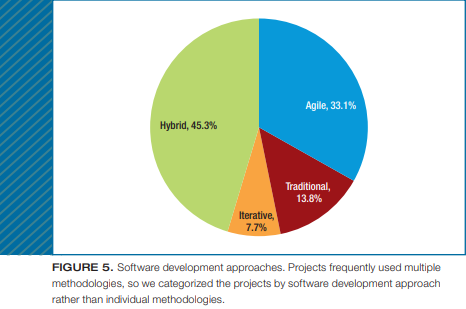
\includegraphics[scale=0.45]{Figures/dm/dm-1.png}}
		\end{figure}

		Figure~\ref{fig:dm-2} by Leo R. Vijayasarathy~\cite{vijayasarathy_choice_2016} shows a comparison of the annual revenue and employee count of each development methodologies by the percentage of companies. This stacked bar chart should help indicate each development methodology's an employee count by company usage; annual fees will not impact the decision to make the development methodology choice as the author states that `The annual revenue wasn’t statistically significant; the number of employees was.'~\cite{vijayasarathy_choice_2016}

		\begin{figure}[H]
			\ffigbox[\FBwidth] {
				\caption[Development Methodology]{Comparison of the annual revenue and employee count of each development methodology (percentage of companies). Leo R. Vijayasarathy~\cite{vijayasarathy_choice_2016}}
				\label{fig:dm-2}
			}
			{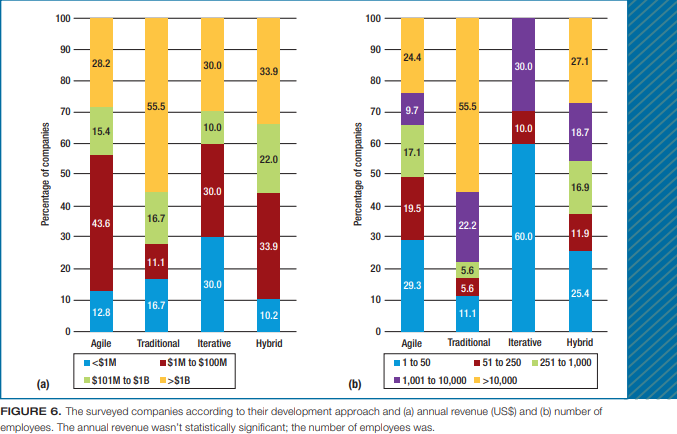
\includegraphics[scale=0.45]{Figures/dm/dm-2.png}}
		\end{figure}

		Figure~\ref{fig:dm-3} by Leo R. Vijayasarathy~\cite{vijayasarathy_choice_2016} shows a comparison of the budget and criticality of each development methodologies by the percentage of projects. This stacked bar chart should help indicate each development methodology's budget and criticality by project usage.
		
		\begin{figure}[H]
			\ffigbox[\FBwidth] {
				\caption[Development Methodology]{Comparison of the budget and criticality of each development methodology (percentage of projects). Leo R. Vijayasarathy~\cite{vijayasarathy_choice_2016}}
				\label{fig:dm-3}
			}
			{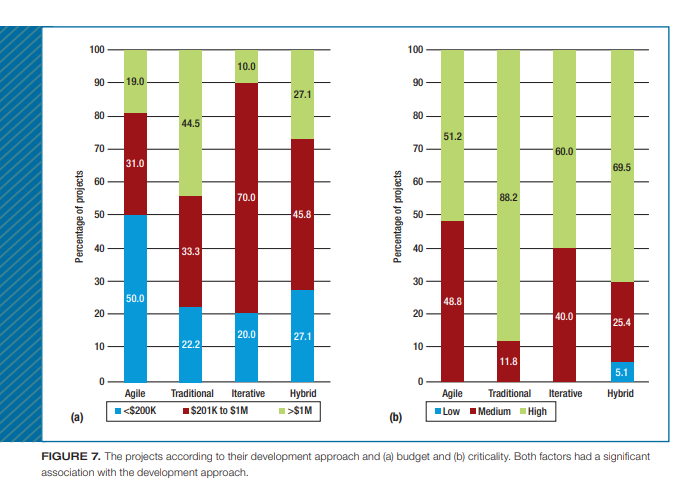
\includegraphics[scale=0.45]{Figures/dm/dm-3.png}}
		\end{figure}

		After observing Figure~\ref{fig:dm-1}, the Hybrid development methodology is the most used for project usage. Agile development methodology comes second, Traditional development methodology comes third, and Iterative development methodology comes fourth. Figure~\ref{fig:dm-2} indicates that the Traditional development methodology requires the most employees to develop projects. The Iterative development methodology requires the least amount of employees to develop projects. Figure~\ref{fig:dm-3} indicates that the Agile development methodology requires less budget and is the most critical. Traditional development methodology requires the highest budget and is the least critical.

		The Iterative development methodology seems to benefit this project for the following reasons:-
		\begin{itemize}
			\item Fewer employees (Fits a individual ran project).
			\item 60\% criticality and 40\% budget (Great balance).
			\item Well-structured development model.
		\end{itemize}

		This development methodology follows the following development steps:-

		\begin{center}
			\scriptsize
			\textbf{Mathematical Key:}\\
			$\mathcal{IP}$: Initial Planning, $\mathcal{C}$: Continue?, $\mathcal{T}$: True, $\mathcal{PL}$: Planning, $\mathcal{RQ}$: Requirements\\$\mathcal{AD}$: Analysis and Design, $\mathcal{IM}$: Implementation, $\mathcal{TT}$: Testing, $\mathcal{EV}$: Evaluation\\$\mathcal{DP}$: Deployment\\
			\textbf{Step 1:}\\
			$\mathcal{IP}$\\
			\textbf{Step 2:}\\ 
			$\mathcal{\sum_{n = 1}^{\mathcal{C\neq}\mathcal{T}}(\mathcal{PL}(\mathcal{RQ} -> \mathcal{AD}) -> \mathcal{IM}_{\mathcal{C}} (\mathcal{TT} -> \mathcal{EV}))}$\\
			\textbf{Step 3:}\\
			$\mathcal{DP}$
		\end{center}

		The Iterative development model will start the Initial Planning, then starts the procedure by going to the Planning stage. The planning stage involves the Requirements and Analysis and Design stage. The implementation stage consists in checking if the project is ready for deployment. If this is not true, this stage involves the Testing and Evaluation stages. The deployment stage is the deployment of the product and the completion state of the project. This stage proceeds on the completion of the implementation. This process is easy to follow, and the repetition of conducting tests and reevaluating the product provides a well-tested end product. However, this process is impractical in a large team environment and can delay the product development time due to the process.

	\chapter{Implementation}
		\section{Main Layout}
			Figure~\ref{fig:guiDesignML-1} is the design implementation of the VisualPro software using Visual Studio. The design starts with two panels, one containing the software's functionality and the other enabling the work area within the software. After examining the design implementation, the software lacked class, function and variable containers to create a code structure.
			\begin{figure}[H]
				\ffigbox[\FBwidth] {
				\caption[GUI Design ML-1]{Design Planning - Stage 1}
				\label{fig:guiDesignML-1}
				}
				{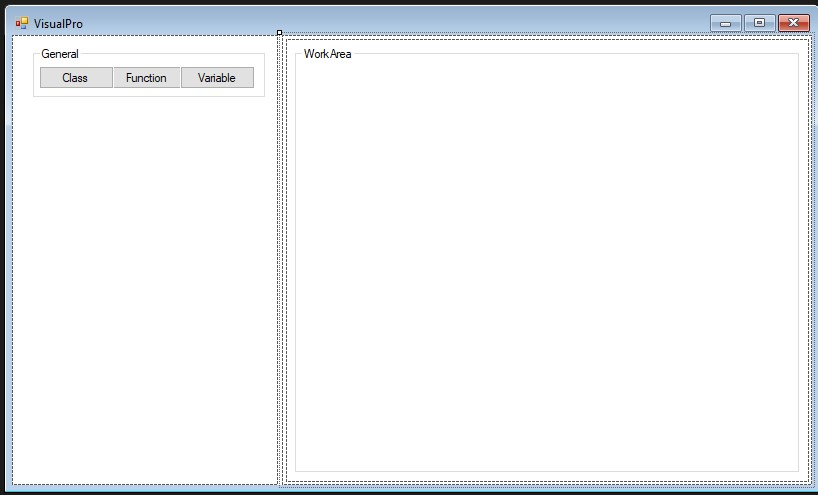
\includegraphics[scale=0.45]{Figures/vp-designs/NET_Framework-GUI-1.jpg}}
			\end{figure}

			After looking at the issues within the first stage, creating a simple class container is now available within the design implementation. However, this time the container seems too basic, and contains zero positioning ideas.
			\begin{figure}[H]
				\ffigbox[\FBwidth] {
				\caption[GUI Design SC-1]{Design Planning - Stage 2}
				\label{fig:guiDesignSC-1}
				}
				{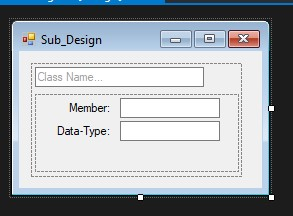
\includegraphics[scale=0.75]{Figures/vp-designs/NET_Framework-GUI-2.jpg}}
			\end{figure}

			From the previous implementation, a design of the container positions provides an idea of how the VisualPro software should enable users to drag containers on the work area. However, the design the positioning of the containers does not generate a good UI and UX design. Another design problem, the software has no options to save the code when the user creates a new project. An extra point to make is that the containers should have access for children and any additional properties.
			\begin{figure}[H]
				\ffigbox[\FBwidth] {
				\caption[GUI Design ML-2]{Design Planning - Stage 3}
				\label{fig:guiDesignML-2}
				}
				{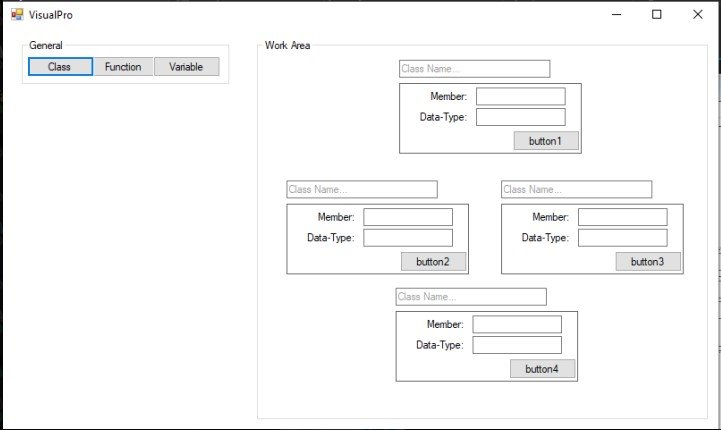
\includegraphics[scale=0.45]{Figures/vp-designs/NET_Framework-GUI-2-1.jpg}}
			\end{figure}

			The previous problem of the last implementation design contains no option to save is now available. The parent and child containers need remaking with a new position scheme for the next iteration. A foreseeable design flaw of Classes, Functions and Variables is that children cannot be higher than their inheritance type during development under the parent container. This problem meant, for example, that the class would be declared inside another class programmatically if the problem occurred under the current logic when the compilation happened. The code syntax makes no sense, resulting in a compilation error. An example of this error within this software could be an \textit{`int variable = int variable;'}. 
			\begin{figure}[H]
				\ffigbox[\FBwidth] {
				\caption[GUI Design ML-3]{Design Planning - Stage 4}
				\label{fig:guiDesignML-3}
				}
				{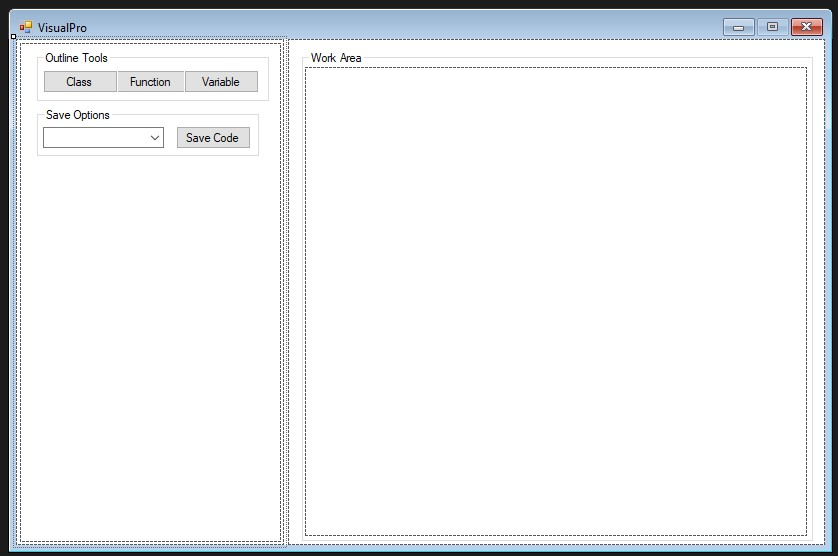
\includegraphics[scale=0.45]{Figures/vp-designs/NET_Framework-GUI-4.jpg}}
			\end{figure}

			Figure~\ref{fig:guiDesignML-4} shows the implementation of the design using the designs shown beforehand. Rather than shortcutting relationships between each class, function and variable by nesting them, the final implementation design prevents the user from dragging and dropping the same type of container onto another container. A property button appears on each container to control function arguments and relationships between classes, functions, and variables, opening up a dialogue containing a property sheet. If any error occurs, there are no error messages or dialogue box designs to alert the user if something is not working as it should be.
			\begin{figure}[H]
				\ffigbox[\FBwidth] {
				\caption[GUI Design ML-4]{Design Planning - Stage 5}
				\label{fig:guiDesignML-4}
				}
				{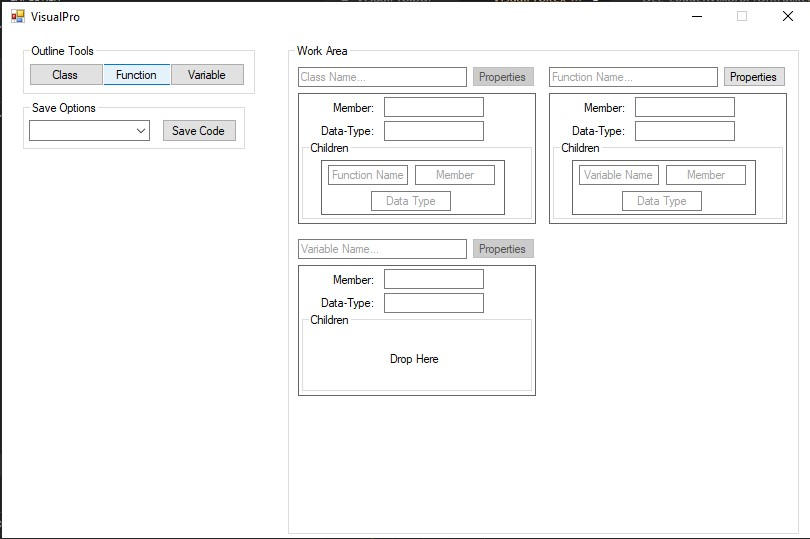
\includegraphics[scale=0.45]{Figures/vp-designs/NET_Framework-GUI-Latest.jpg}}
			\end{figure}
		
		\section{Error Handling}
			The previous iteration implementation design problem, `Error Dialogue,' is now available. This dialogue design helps inform the user if the software fails. The dialogue only activates if there is a syntax language error within the `VisualPro.xml' language configuration file. This design should expand to include other errors that occur within the software.
			\begin{figure}[H]
				\ffigbox[\FBwidth] {
				\caption[GUI Design EH-1]{Error Handling}
				\label{fig:guiDesignEH-1}
				}
				{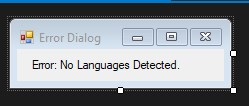
\includegraphics[scale=0.75]{Figures/vp-designs/NET_Framework-GUI-ErrorDialog.jpg}}
			\end{figure}
		
	\chapter{Evaluation of Functionality}
		During the development of VisualPro, a few unit tests to test mainly the backend would give some idea of evaluation of the functionality. These tests will cross-reference with the front-end implementation to establish whether the lack of functionality comes down to the front-end or the backend implementation. Any bugs found should list within the tutorial to help any new developers navigate VisualPro without hitting the same known bugs.

		\section{Decoder Tools}
			Tools to parse encrypted strings of characters full of information to decipher particular information help the communication between the front-end and the backend. In some cases, tool functionality developed within C\# for the VisualPro software seems to slow down the software, so in extreme cases, redevelopment with the C++ language of these tools to use in the VisualPro software increased the performance of the software.

			`FindSubStrA' is a test that searches for a word between two characters. The function (originally in C\#) asks for a start \textbf{(char)}, end \textbf{(char)}, position \textbf{(int)}, and a string \textbf{(std::string)} to make this search possible. All the tests within `FindSubStrA' are successful.

			\begin{lstlisting}[language=c++]
				TEST_METHOD(FindSubStrA)
				{
					/* Error Log:
					* All tests passed.
					* Purpose of tool is to find a word between two characters.
					*/
					// Seperators: | |
					Assert::AreEqual("H", CSFindSubStr('|', '|', 0, "|H|E-L-LxO").c_str());

					// Seperators: | -
					Assert::AreEqual("E", CSFindSubStr('|', '|', 1, "|H|E|L-LxO").c_str());

					// Seperators: - -
					Assert::AreEqual("L", CSFindSubStr('-', '-', 0, "|H|E-L-LxO").c_str());

					// Seperators: - -
					Assert::AreEqual("L", CSFindSubStr('-', 'x', 1, "|H|E-L-LxO").c_str());

					// Seperators: - \0
					Assert::AreEqual("O", CSFindSubStr('x', '\0', 0, "|H|E-L-LxO").c_str());
				}
			\end{lstlisting}

			`FindSubStrB' tests the C++ version of the previous function. This time it checks for a separator and position. The arguments to find a separated substring, string \textbf{(const char*)}, string to test \textbf{(const char*)}, separator \textbf{(char)} and position \textbf{(int)}. One test passed, and the other two failed. This test problem is one of the reasons why the code generation does not generate properly. Without this test, it would have been hard to decipher the survey code submitted further down.

			\begin{lstlisting}[language=c++]
				TEST_METHOD(FindSubStrB)
				{
					/* Error Log:
					* Test A - Failed -> Test Written Wrongly | Passed
					* Test B - Passed
					* Test C - Failed -> Selects Each Word | Temporary Solution: Read Below.
					*/

					// Seperator |
					// Checks all words. - Test A
					for (size_t i = 0; i < 3; i++)
						Assert::AreEqual(("Word " + std::to_string(i + 1)).c_str(), CPPFindSubStr("Word 1|Word 2|Word 3", "Word", '|', i).c_str());

					// Finds First Word - Test B
					// Seperator x
					Assert::AreEqual("A", CPPFindSubStr("AxYZxQRxAxB", "A", 'x', 0).c_str());

					// Finds First Word in Each Position - Test C
					// Seperator x

					// current status: Fail (selects each word) - Temporary solution:
					// if(word == "A") or further rework
					std::string word = std::string();
					for (size_t i = 0; !(word = CPPFindSubStr("AxYZxQRxAxB", "A", 'x', (int)i)).empty(); i++)
						if (word == "A")
							Assert::AreEqual("A", word.c_str());
				}
			\end{lstlisting}

			`FindStrIndexA' test will observe the substring index from a set of arguments. The functionality enables the developer to find an index of a string's character. The function requires two arguments, string \textbf{(const char*)} and test subject \textbf{(char)}. All parts of the test passed.
			\begin{lstlisting}[language=c++]
				TEST_METHOD(FindStrIndexA)
				{
					/* Error Log:
					* Test A - Passed
					* Test B - Passed
					* Test C - Passed
					*/

					//Expectation: 6 | Test A
					Assert::AreEqual(6, FindStrIndex("!)2pAL@sSwS", '@'));
					//Expectation: Not -1 && is 8 | Test B
					Assert::AreNotEqual(-1, FindStrIndex("!)2pAL!sSwS", 'S'));
					Assert::AreEqual(8, FindStrIndex("!)2pAL!sSwS", 'S'));


					// Expectation: -1 | Test C
					Assert::AreEqual(-1, FindStrIndex("!)2pAL!sSwS", '~'));
					Assert::AreEqual(-1, FindStrIndex("!)2pAL!sSwS", '1'));
					Assert::AreEqual(-1, FindStrIndex("!)2pAL!sSwS", 'M'));
				}
			\end{lstlisting}

			`ReplaceWordA' tests the replace string by a substring. The function requires five arguments, string \textbf{(const char*)}, depth \textbf{(int)}, start \textbf{(char)}, end \textbf{(char)} and replaceString \textbf{(const char*)}. All tests passed.
			\begin{lstlisting}[language=c++]
				TEST_METHOD(ReplaceWordA)
				{
					/* Error Log
					* 
					*/
					const std::string aMistake = "A:Banana\x1f\B:Pineapple\x1f\C:Grapefruit",
						testA = ReplaceWord(aMistake.c_str(), 1, ':', '\x1f', "Apple"),
						testB = ReplaceWord(testA.c_str(), 3, ':', '\x1f', "Banana");
					const char* expected = "A:Apple\x1f\B:Pineapple\x1f\C:Grapefruit",
								*secExpected = "A:Apple\x1f\B:Pineapple\x1f\C:Banana";

					Assert::AreNotEqual(expected, aMistake.c_str());
					Assert::AreEqual(expected, testA.c_str());
					Assert::AreEqual(secExpected, testB.c_str());
				}
			\end{lstlisting}
		\section{Lists}
			VisualPro communicates to the Programming Planner library using C++ `Lists' class. Without the `List' class functionality testing, many errors that could be down to the `Lists' class or front-end implementation would make this project impossible to create. Three important functionality of `Lists' class are the `GetSignature', `Addition' and `Deletion' functions. The signature signifies whether an item is a Class, Function, Argument or Variable to the Programming Planner.
            
            The `List\_Addition' enables the addition of Lists. The test examines the addition of an item and passes the first try. When creating the VisualPro software, any communication issues would lay on the front-end side.

			\begin{lstlisting}[language=c++]
				TEST_METHOD(List_Addition)
				{
					/* Error Log:
						First Try: Pass - (A, B, C, D, E, F, G, H)
					*/

					// Creation of a new list with X, on addition the ID's should follow as X-1, X-2 etc.
					List* xList = new List("X");
					List* yList = new List("Y"); // Same but Y-1, Y-2 etc.
					List* xyList = new List("XY"); // XY-1, XY-2 etc.

					// Should return X - Test | A
					Assert::AreEqual("X", xList->GetSignature().c_str());

					// Should return Y - Test | B
					Assert::AreEqual("Y", yList->GetSignature().c_str());

					// Should return XY - Test | C
					Assert::AreEqual("XY", xyList->GetSignature().c_str());

					// Should return X-1 - Test | D
					Assert::AreEqual("X-1", xList->Add("parentItem"));

					// Should return Y-1\x1fP-X-1 - Test | E
					Assert::AreEqual("Y-1\x1fP-X-1", yList->Add("childItem", "X-1"));

					// Should return Y-2 - Test | F
					Assert::AreEqual("Y-2", yList->Add("parentItem"));

					// Should return X-2 - Test | G
					Assert::AreEqual("X-2", xList->Add("parentItem"));

					// Should return XY-1 - Test | H
					Assert::AreEqual("XY-1\x1fP-X-2", xyList->Add("parentItem", "X-2"));

					// Garbage collection for the test.
					delete xList; delete yList; delete xyList;
				}
			\end{lstlisting}

			VisualPro tries to offer as much functionality as possible, including container removal. This functionality will not work if the code generator generates the same items, where `List\_Deletion' comes into play. The `List\_Deletion' tests the list deletion. The test passes the first try.

			\begin{lstlisting}[language=c++]
				TEST_METHOD(List_Deletion)
				{
					/* Error Log:
					* First Try: Pass
					*/

					// Creation of X
					List* list = new List("X");
					list->Add("Function 1"); // ID: X-1
					list->Add("Function 2"); // ID: X-2
					list->Add("Function 3"); // ID: X-3

					// Both work but top is more tidy and saves some memory
					// History: Design of List was originally for displaying on Console and therefore saves any extra logic after calling ListAll method.
					// Ideal - Test | A-I:
					Assert::AreNotEqual("X-1  Function 1\nX-2  Function 2\nX-3  Function 3", list->ListAll().c_str());
					// Actual - Test | A-A: 
					Assert::AreEqual("X-1  Function 1  \nX-2  Function 2  \nX-3  Function 3  \n\n", list->ListAll().c_str());

					list->Remove(2); // Expectation: Function 2 goes disappears

					// To test if removal of List works - Test | B
					Assert::AreEqual("X-1  Function 1  \nX-3  Function 3  \n\n", list->ListAll().c_str());

					// Performance Improvement 
					// Ideal - It would be ideal to replace a empty ID (X-2 is non-existent, though X-4 is next) - Test | C-I
					Assert::AreNotEqual("X-2", list->Add("Method 2")); // The list should fill in the empty ID to save data.

					Assert::AreEqual("X-1  Function 1  \nX-3  Function 3  \nX-4  Method 2  \n\n", list->ListAll().c_str());

					// However, if the last element is non existence, the ID will rollback to any previously unique ID's that are not taken by the last element.)
					// Which, in theory provides short IDs that are suitable for Programming Planner's solution.
					// Actual - Test | D-A
					list->Remove(2);
					list->Remove(3);
					list->Remove(4);
					Assert::AreEqual("X-2", list->Add("Method 2"));

					delete list;
				}
			\end{lstlisting}

	\chapter{Evaluation of Feedback}
		\section{Programmer Planner vs. VisualPro}
			Figure~\ref{fig:EoF-SQ-A1}: Two respondents, 33.3\%, have experience with Programming Planner previously. These candidates will help compare the two programs. Within the first question, `What program delivered better user experience?' - zero being Programming Planner and ten being VisualPro. The two respondents range from option nine to ten, indicating that they prefer VisualPro to Programming Planner as a development tool.

			\begin{figure}[H]
				\ffigbox[\FBwidth] {
				\caption[Evaluation of Feedback - SQ-A1]{Evaluation of Feedback - SQ-A1}
				\label{fig:EoF-SQ-A1}
				}
				{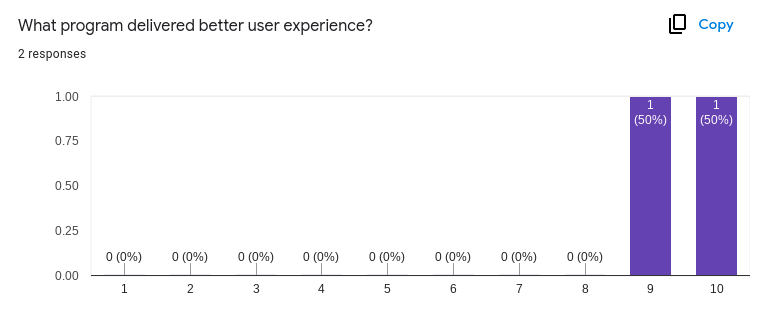
\includegraphics[scale=0.50]{Figures/VisualPro-Survey_Results/SQ-A1.png}}
			\end{figure}

			Figure~\ref{fig:EoF-SQ-A2}: `Which software ticks your boxes for a development tool?', has four attributes, `Ease of Use', `Performance', `Extra Features' and `File Structure', and allows the respondents to choose Programming Planner or VisualPro. The key within figure~\ref{fig:EoF-SQ-A2} indicates whether the respondents chose Programming Planner or VisualPro. The respondents chose VisualPro for each attribute.

			\begin{figure}[H]
				\ffigbox[\FBwidth]{
					\caption[Evaluation of Feedback - SQ-A2]{Evaluation of Feedback - SQ-A2}
					\label{fig:EoF-SQ-A2}
				}
				{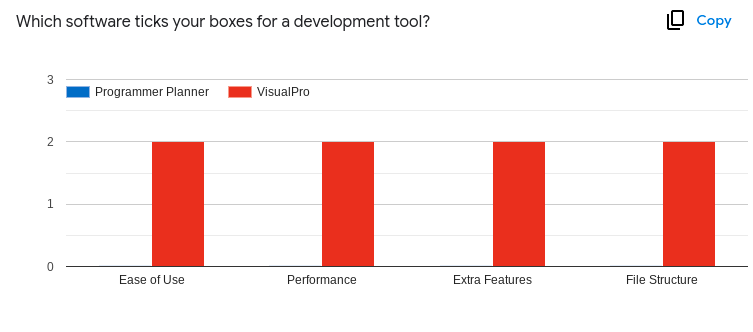
\includegraphics[scale=0.50]{Figures/VisualPro-Survey_Results/SQ-A2.png}}
			\end{figure}

			Figure~\ref{fig:EoF-SQ-A3}: `Does VisualPro improve the user experience instead of Programming Planner?', all respondents chose `Yes', displaying that the respondents feel VisualPro made improvements to the UX from the Programming Planner software.

			\begin{figure}[H]
				\ffigbox[\FBwidth]{
					\caption[Evaluation of Feedback - SQ-A3]{Evaluation of Feedback - SQ-A3}
					\label{fig:EoF-SQ-A3}
				}
				{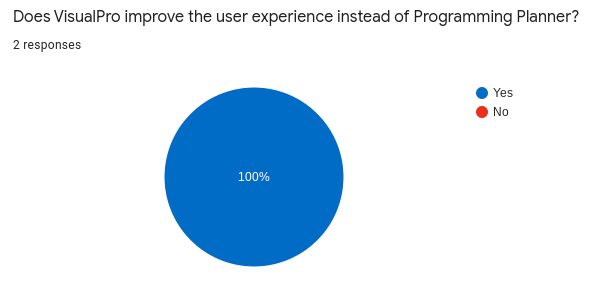
\includegraphics[scale=0.50]{Figures/VisualPro-Survey_Results/SQ-A3.png}}
			\end{figure}

			Figure~\ref{fig:EoF-SQ-A4}: `Which program is more beginner friendly?' measured on a scale of one (Programming Planner) to ten (VisualPro). Half of the respondents chose eight, and the other half chose ten. This result suggests that VisualPro is more beginner-friendly than Programming Planner.

			\begin{figure}[H]
				\ffigbox[\FBwidth]{
					\caption[Evaluation of Feedback - SQ-A4]{Evaluation of Feedback - SQ-A4}
					\label{fig:EoF-SQ-A4}
				}
				{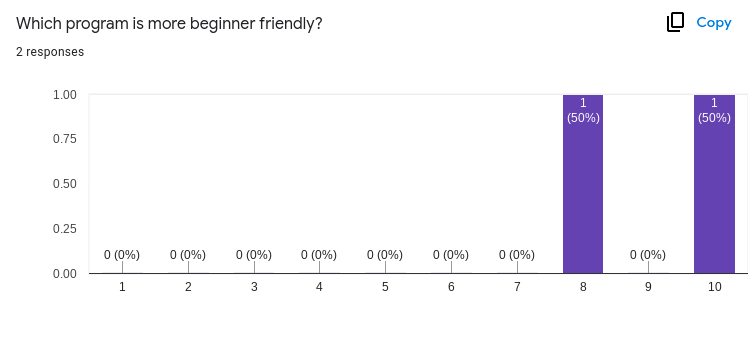
\includegraphics[scale=0.50]{Figures/VisualPro-Survey_Results/SQ-A4.png}}
			\end{figure}

			Figure~\ref{fig:EoF-SQ-A5}: `Does the software provide enough tuitive ways to create structure?' half of the respondents chose `Yes', and the other half chose `No'. This response demonstrates that the software could do with more functionality to provide a better-structured environment with remarkable UX and User Usability.

			\begin{figure}[H]
				\ffigbox[\FBwidth]{
					\caption[Evaluation of Feedback - SQ-A5]{Evaluation of Feedback - SQ-A5}
					\label{fig:EoF-SQ-A5}
				}
				{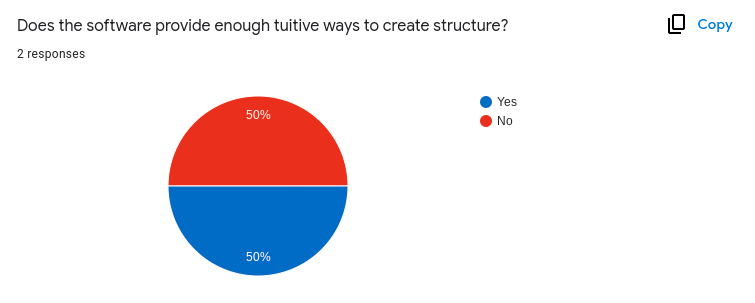
\includegraphics[scale=0.50]{Figures/VisualPro-Survey_Results/SQ-A5.png}}
			\end{figure}

			`List any unknown bugs and provide steps', listed responses:
			\begin{itemize}
				\item `The end code that was generated need more configuaration.'
				\item `havent found any'.
			\end{itemize}

		\section{VisualPro}
			This section includes all the six respondents. Two of these respondents have prior experience with testing VisualPro and Programming Planner. The marking scheme analyses if the code generation is correct to the example shown within the tutorial, partially correct; due to bugs or other issues or not correct. This data would be passed through a Fuzzy Expert Logic algorithm to determine the overall User Usability.
			\subsection{Object-Oriented Programming - Tutorial A | Exercise: Creating a Class}
				This section of Tutorial A aims to create a' World' class. The initial question of this section, `Write your understanding of a Class from what you have learnt from Tutorial A', listed responses:
				\begin{itemize}
					\item `I have learnt and used the class as a container and used it with ease in VisualPro.'
					\item `A way to contain code to use later on'.
					\item `a class enables developers to containerise code that can be referenced later as an object.'
					\item `A class is code that is containerised so it can be referenced at a later stage as an object.'
					\item `Classes provide developers with the ability to use a string syntax in object-oriented environments'.
					\item `A way to group blocks of code'.
				\end{itemize}

				Figure~\ref{fig:EoF-SQ-BAA1}: `Rate the ease of creating a Class within VisualPro' on a one (understandable) to ten (Incomprehensible) scale. 33.3\% of the respondents chose one, 16.7\% chose two, 33.3\% chose three, and 16.7\% chose five. This data could imply that the structure is not quite there yet, and it is essential to focus on the UX and User Usability of the existing features before adding more.

				\begin{figure}[H]
					\ffigbox[\FBwidth]{
						\caption[Evaluation of Feedback - SQ-BAA1]{Evaluation of Feedback - SQ-BAA1}
						\label{fig:EoF-SQ-BAA1}
					}
					{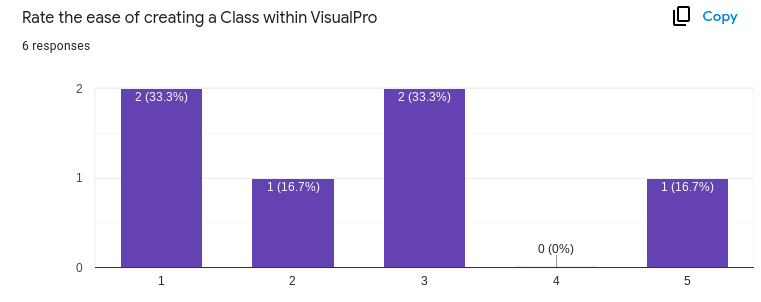
\includegraphics[scale=0.50]{Figures/VisualPro-Survey_Results/SQ-BAA1.png}}
				\end{figure}

				Figure~\ref{fig:EoF-SQ-BAA2}: `Did your VisualPro Work Area look identical to the example shown?', 66.7\% respondents chose `Yes', 33.3\% chose `No'. This response points out that four code generations are correct and the others are not.
				\begin{figure}[H]
					\ffigbox[\FBwidth]{
						\caption[Evaluation of Feedback - SQ-BAA2]{Evaluation of Feedback - SQ-BAA2}
						\label{fig:EoF-SQ-BAA2}
					}
					{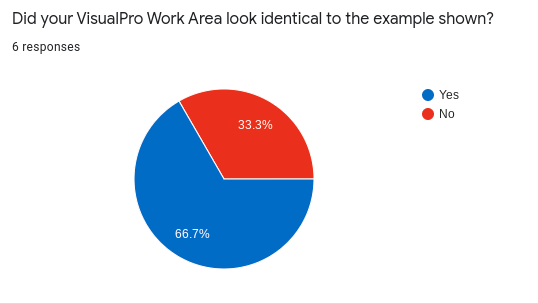
\includegraphics[scale=0.50]{Figures/VisualPro-Survey_Results/SQ-BAA2.png}}
				\end{figure}

				`Your Code Snippet', listed responses:
				
				\textit{First Response:} 
				\begin{lstlisting}[language=c++]
					#include <iostream>
					#include <string>
					
					class name
					{
						class-1
					};
				\end{lstlisting} - This respondent seems to have followed this task correctly.

				\textit{Second Response:}
				\begin{lstlisting}[language=c++]
					#include <iostream>

					#include <string>

					class name
					{
						class-1
					};
				\end{lstlisting} - This respondent seems to have followed this task correctly.

				\textit{Third Response:}
				\begin{lstlisting}[language=java]
					class World {

					};
				\end{lstlisting} - This respondent followed this task correctly.

				\textit{Fourth Response:}
				\begin{lstlisting}[language=c++]
					class Name {
						protected :
							void Method () {}
						public :
							void Method () {}
						private :
							void Method () {}
					};
				\end{lstlisting} - This respondent followed this task incorrectly.

				\textit{Fifth Response:}
				\begin{lstlisting}[language=c++]
					#include <iostream>
					#include <string>

					class World
					{
						class-1
					};
				\end{lstlisting} - This respondent followed this task correctly.

				\textit{Sixth Response:}
				\begin{lstlisting}[language=c++]
					#include <iostream>
					#include <string>

					class name
					{
						class-1
					};
				\end{lstlisting} - This respondent seems to have followed this task correctly.

			\subsection{Object-Oriented Programming - Tutorial A | Exercise: Animal Types}
			The aim of this tutorial is to create different Animal classes to get use to OOP style structures. The question `What main methods/variables separate Reptiles, Mammals and Amphibians from one another?' aims to test the respondents ability to select the correct details within OOP style prorgamming. The following responses were given:
			\begin{itemize}
				\item `amimal type?'.
				\item `sound'.
				\item `Class'.
				\item `Method Name'.
			\end{itemize}

			Two out of four responses chose a reasonable answer; these are `animal type?' and `sound'. The last two may or may not have confused the question and tried to answer the question by OOP terminology. The responses are fair and may suggest that the tutorial helped the respondents to understand OOP style programming or think of a different way of describing OOP style programming. Two out of four responses chose a reasonable answer; these are `animal type?' and `sound'. The last two may or may not have confused the question and tried to answer the question by OOP terminology.

			Figure~\ref{fig:EoF-SQ-BAB1}: `Did your VisualPro Work Area look identical to the example shown?', 66.7\% respondents chose `Yes', 33.3\% chose `No'. This response points out that four code generations are correct and the others are not.

			\begin{figure}
				\ffigbox[\FBwidth]{
					\caption[Evaluation of Feedback - SQ-BAB1]{Evaluation of Feedback - SQ-BAB1}
					\label{fig:EoF-SQ-BAB1}
				}
				{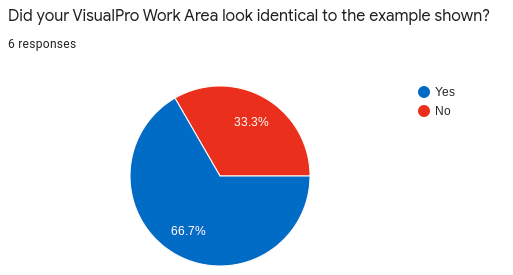
\includegraphics[scale=0.50]{Figures/VisualPro-Survey_Results/SQ-BAB1.png}}
			\end{figure}

			`Your Code Snippet', listed responses:

			\textit{First Response:}
			\begin{lstlisting}[language=c++]
				class Reptile {

				};

				class Mammals {

				};

				class Amphibian {

				};
			\end{lstlisting} - This respondent followed this task correctly.

			\textit{Second Response:}
			\begin{lstlisting}[language=c++]
				#include <iostream>
				#include <string>

				class name
				{
					class-1
				};

				class name
				{
					class-2
				};

				class name
				{
					class-3
				};
			\end{lstlisting} - This respondent seems to have followed this task correctly.

			\textit{Third Response:}
			\begin{lstlisting}[language=c++]
				#include <iostream>
				#include <string>

				class name
				{
					class-1
				};

				class name
				{
					class-2
				};

				class name
				{
					class-3
				};

				class name
				{
					class-4
				};
			\end{lstlisting} - This respondent seems to have followed this task correctly.

			\textit{Fourth Response:}
			\begin{lstlisting}[language=c++]
				#include <iostream>
				#include <string>

				class name
				{
					class-1
				};

				class name
				{
					class-2
				};

				class name
				{
					class-3
				};
			\end{lstlisting} - This respondent seems to have followed this task correctly.

			\textit{Fifth Response:}
			\begin{lstlisting}[language=c++]
				class Name {
				protected :
					void Method () {}
				public :
					void Method () {}
				private :
					void Method () {}
				};
			\end{lstlisting} - This respondent followed this task incorrectly.

			\textit{Sixth Response:}
			\begin{lstlisting}[language=c++]
				#include <iostream>
				#include <string>

				class name
				{
					class-1
				};

				class name
				{
					class-2
				};

				class name
				{
					class-3
				};
			\end{lstlisting} - This respondent seems to have followed this task correctly.

			\subsection{Tutorial A | Exercise: Vehicle Components}
				The objective of this exercise is to ask the respondents to think of a few vehicle components and their corresponding methods, whilst implmentating the product into VisualPro. Figure~\ref{fig:EoF-SQ-BAC1}: `Did your VisualPro Work Area look identical to the example shown?', 66.7\% respondents chose `Yes', 33.3\% chose `No'. This response points out that four code generations are correct and the others are not.

				\begin{figure}[H]
					\ffigbox[\FBwidth]{
						\caption[Evaluation of Feedback - SQ-BAC1]{Evaluation of Feedback - SQ-BAC1}
						\label{fig:EoF-SQ-BAC1}
					}
					{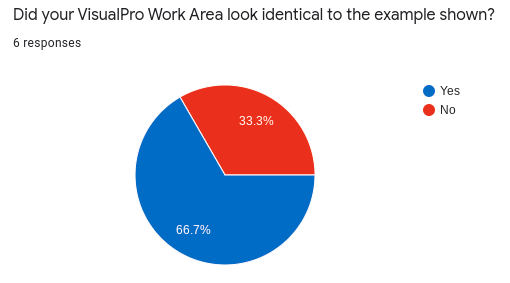
\includegraphics[scale=0.50]{Figures/VisualPro-Survey_Results/SQ-BAC1.png}}
				\end{figure}
				
				`Your Code Snippet', listed responses:

				\textit{First Response:}
				\begin{lstlisting}[language=c++]
					class Engine {
					};

					class Wheel {
					};
				\end{lstlisting} - This respondent followed this task correctly.

				\textit{Second Response:}
				\begin{lstlisting}[language=c++]
					#include <iostream>

					#include <string>

					dt name()
					{
						function-1
					}

					dt name
				\end{lstlisting} - This respondent followed this task incorrectly.

				\textit{Third Response:}
				\begin{lstlisting}[language=c++]
					#include <iostream>
					#include <string>

					class name
					{
						class-1
					};

					class name
					{
						class-2
					};

					class name
					{
						class-3
					};

					class name
					{
						class-4
					};

					class name
					{
						class-5
					};

					dt namedt namedt namedt name
				\end{lstlisting} - This respondent seems to have followed this task correctly.

				\textit{Fourth Response:}
				\begin{lstlisting}[language=java]
					Public class name
					{
						class-1
					}
					
					dt name()
					{
						function-1
					}
					
					dt name()
					{
						function-2
					}
					
					dt name()
					{
						function-3
					}
				\end{lstlisting} - This respondent seems to have followed this task correctly.

				\textit{Fifth Response:}
				\begin{lstlisting}[language=c++]
					.
				\end{lstlisting} - This respondent followed this task incorrectly.

				\textit{Sixth Response:}
				\begin{lstlisting}[language=java]
					member class name
					{
						class-1
					}

					member class name
					{
						class-2
					}

					member class name
					{
						class-3
					}

					dt name()
					{
						function-1
					}

					dt name()
					{
						function-2
					}

					dt name()
					{
						function-3
					}

					dt name()
					{
						function-1
					}

					dt namedt name
				\end{lstlisting} - This respondent seems to have followed this task correctly.

			\subsection{Object-Oriented Programming - Tutorial A | Exercise: Try It Yourself (TIY)}
				This exercise allows the respondents to get creative and try creating some OOP scenarios of their own. Figure~\ref{fig:EoF-SQ-BAD1}: `Did your VisualPro Work Area look identical to the example shown?', 66.7\% respondents chose `Yes', 33.3\% chose `No'. This response points out that four code generations are correct and the others are not.
				
				\begin{figure}[H]
					\ffigbox[\FBwidth]{
						\caption[Evaluation of Feedback - SQ-BAD1]{Evaluation of Feedback - SQ-BAD1}
						\label{fig:EoF-SQ-BAD1}
					}
					{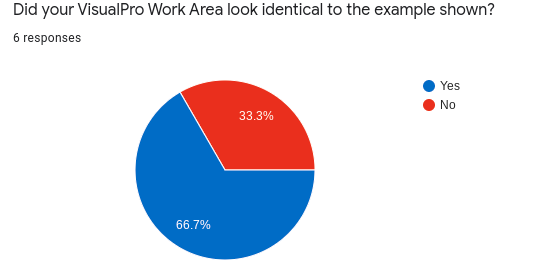
\includegraphics[scale=0.50]{Figures/VisualPro-Survey_Results/SQ-BAD1.png}}
				\end{figure}

				`Your Code Snippet', listed responses:
				\textit{First Response:}
				\begin{lstlisting}[language=c++]
					class Planet {
					};

					class Computer {
					};
				\end{lstlisting} - This respondent followed this task correctly.

				\textit{Second Response:}
				\begin{lstlisting}[language=c++]
					#include <iostream>
					#include <string>

					class Computer
					{
						class-1
					};
				\end{lstlisting} - This respondent followed this task correctly.

				\textit{Third Response:}
				\begin{lstlisting}[language=c++]
					n/a
				\end{lstlisting} - This respondent followed this task incorrectly.

				\textit{Fourth Response:}
				\begin{lstlisting}[language=java]
					using System;

					public class name
					{
					class-1
					}

					dt name
				\end{lstlisting} - This respondent followed this task correctly.

				\textit{Fifth Response:}
				\begin{lstlisting}[language=c++]
					.
				\end{lstlisting} - This respondent followed this task incorrectly.

				\textit{Sixth Response:}
				\begin{lstlisting}[language=java]
					member class name
					{
						class-1
					}

					member class name
					{
						class-2
					}

					member class name
					{
						class-3
					}

					dt name()
					{
						function-1
					}

					dt name()
					{
						function-2
					}

					dt name()
					{
						function-3
					}

					dt name()
					{
						function-1
					}

					dt namedt name
				\end{lstlisting} - This respondent seems to have followed this task correctly.

			\subsection{Functional Programming - Tutorial B | Exercise: Toaster Functionality}
				`Toaster Functionality' exercise is to establish the functionality of a toaster to get grips of FP style programming. The initial question, `What is the difference between OOP and FP styles?' helps understand if the respondents' have learnt the complexity of the two styles. Responses of the respondents:

				\begin{itemize}
					\item `I personally found less code but the oop style is easier to read.'
					\item `oop focuses on user objects over functional approach'.
					\item `not sure'.
					\item `FP uses a fixed data structure, while OOP applies a variable one.'
					\item `OOP enables object creation. FP style contains functional structure.'
					\item `OOP is more dynamic compared to the FP which is more structured'.
				\end{itemize} - Generally speaking, the respondents have learned the differences between both styles throughout the tutorials and VisualPro experience.

				Figure~\ref{fig:EoF-SQ-BBA1}: `Was creating an FP style structure than traditional methods?', 83.3\% respondents chose `Yes', 16.7\% chose `No'. This question tries to figure out if using VisualPro makes it easier implementating FP style programming over traditional methods. The responses indicate that VisualPro seems to make structure programming easier over typing out structure in FP style. However, bare in mind that these respondents may or may have not touched any type of programming language previously.

				\begin{figure}[H]
					\ffigbox[\FBwidth]{
						\caption[Evaluation of Feedback - SQ-BBA1]{Evaluation of Feedback - SQ-BBA1}
						\label{fig:EoF-SQ-BBA1}
					}
					{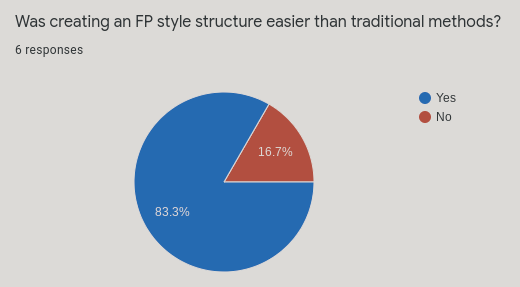
\includegraphics[scale=0.50]{Figures/VisualPro-Survey_Results/SQ-BBA1.png}}
				\end{figure}

				Figure~\ref{fig:EoF-SQ-BBA2}: `Did your VisualPro Work Area look identical to the example shown?', 66.7\% respondents chose `Yes', 33.3\% chose `No'. This response points out that four code generations are correct and the others are not.

				\begin{figure}[H]
					\ffigbox[\FBwidth]{
						\caption[Evaluation of Feedback - SQ-BBA2]{Evaluation of Feedback - SQ-BBA2}
						\label{fig:EoF-SQ-BBA2}
					}
					{\includegraphics[scale=0.50]{Figures/VisualPro-Survey_Results/SQ-BBA2.png}}
				\end{figure}
				
				`Your Code Snippet', listed responses:

				\textit{First Response:}
				\begin{lstlisting}[language=c++]
					#include <iostream>

					#include <string>

					dt name()
					{
						function-1
					}

					dt name()
					{
						function-2
					}

					dt name()
					{
						function-3
					}
				\end{lstlisting} - This respondent seems to have followed this task correctly.

				\textit{Second Response:}
				\begin{lstlisting}[language=c++]
					not sure
				\end{lstlisting} - This respondent followed this task incorrectly.

				\textit{Third Response:}
				\begin{lstlisting}[language=c++]
					class name
					{
						class-1
					};

					class name
					{
						class-2
					};

					class name
					{
						class-3
					};

					class name
					{
						class-4
					};

					class name
					{
						class-5
					};

					dt name()
					{
						function-1
					}

					dt name()
					{
						function-2
					}

					dt name()
					{
						function-3
					}

					dt namedt namedt namedt name
				\end{lstlisting} - This respondent followed this task incorrectly.

				\textit{Fourth Response:}
				\begin{lstlisting}[language=c]
					# include < stdio .h >
					// Declaration
					float XMultiplyY ( double x , double y ) ;
					int main (int argc , char ** argv ) {
					printf (" 8.87 * 2.65 = %f", XMultiplyY (8.87 , 2.65) ) ;
					// result : 23.505501
					return 0;
					}
					// Definition
					float XMultiplyY ( double x , double y ) {
					return x * y
				\end{lstlisting} - This respondent followed this task incorrectly.

				\textit{Fifth Response:}
				\begin{lstlisting}[language=c++]
					#include <iostream>
					#include <string>

					dt name()
					{
						function-1
					}

					dt name()
					{
						function-2
					}

					dt name()
					{
						function-3
					}
				\end{lstlisting} - This respondent seems to have followed this task correctly.

				\textit{Sixth Response:}
				\begin{lstlisting}[language=c++]
					#include <iostream>
					#include <string>

					dt name()
					{
						function-1
					}

					dt name()
					{
						function-2
					}

					dt name()
					{
						function-3
					}
				\end{lstlisting} - This respondent seems to have followed this task correctly.

			\subsection{Functional Programming - Tutorial B | Exercise: Toaster Variables}
				The purpose of this exercise is to test the respondents on the ability of selecting Toaster Variables. These can vary from temperature, timers and other variables. Figure~\ref{fig:EoF-SQ-BBB1}: `Did your VisualPro Work Area look identical to the example shown?', 66.7\% respondents chose `Yes', 33.3\% chose `No'. This response points out that four code generations are correct and the others are not.

				\begin{figure}[H]
					\ffigbox[\FBwidth]{
						\caption[Evaluation of Feedback - SQ-BBB1]{Evaluation of Feedback - SQ-BBB1}
						\label{fig:EoF-SQ-BBB1}
					}
					{\includegraphics[scale=0.50]{Figures/VisualPro-Survey_Results/SQ-BBB1.png}}
				\end{figure}

				`Your Code Snippet', listed responses:

				\textit{First Response:}
				\begin{lstlisting}[language=c++]
					#include <iostream>
					#include <string>

					dt namedt name
				\end{lstlisting} - This respondent seems to have followed this task correctly.

				\textit{Second Response:}
				\begin{lstlisting}[language=c++]
					#include <iostream>
					#include <string>

					dt name()
					{
						function-1
					}

					dt name()
					{
						function-2
					}

					dt name()
					{
						function-3
					}
				\end{lstlisting} - This respondent followed this task incorrectly.

				\textit{Third Response:}
				\begin{lstlisting}[language=c++]
					#include <iostream>
					#include <string>

					dt name()
					{
						function-1
					}

					dt namedt namedt name
				\end{lstlisting} - This respondent seems to have followed this task correctly.

				\textit{Fourth Response:}
				\begin{lstlisting}
					class name
					{
						class-1
					};

					class name
					{
						class-2
					};

					class name
					{
						class-3
					};

					class name
					{
						class-4
					};

					class name
					{
						class-5
					};

					dt name()
					{
						function-1
					}

					dt name()
					{
						function-2
					}

					dt name()
					{
						function-3
					}

					dt namedt namedt namedt name
				\end{lstlisting} - This respondent followed this task incorrectly.

				\textit{Fifth Response:}
				\begin{lstlisting}[language=c++]
					float temperature ;
					int timer;
				\end{lstlisting} - This respondent followed this task correctly.

				\textit{Sixth Response:}
				\begin{lstlisting}[language=c++]
					#include <iostream>
					#include <string>

					dt namedt name
				\end{lstlisting} - This respondent seems to have followed this task correctly.
			

			\subsection{Functional Programming - Tutorial B | Exercise: Fuel Station}
				The `Fuel Station' exercise provides some direction. As long as the respondent can identify \textbf{\textit{any}} functions or variables within a Fuel Station indicates that they are following the task correctly. Figure~\ref{fig:EoF-SQ-BBC1}: `Did your VisualPro Work Area look identical to the example shown?', 66.7\% respondents chose `Yes', 33.3\% chose `No'. This response points out that four code generations are correct and the others are not.
				
				\begin{figure}[H]
					\ffigbox[\FBwidth]{
						\caption[Evaluation of Feedback - SQ-BBC1]{Evaluation of Feedback - SQ-BBC1}
						\label{fig:EoF-SQ-BBC1}
					}
					{\includegraphics[scale=0.50]{Figures/VisualPro-Survey_Results/SQ-BBC1.png}}
				\end{figure}

				`Your Code Snippet', listed responses:

				\textit{First Response:}
				\begin{lstlisting}[language=c++]
					#include <iostream>
					#include <string>

					dt name()
					{
						function-1
					}

					dt name()
					{
						function-2
					}

					dt name()
					{
						function-3
					}

					dt name
				\end{lstlisting} - This respondent seems to have followed this task correctly.

				\textit{Second Response:}
				\begin{lstlisting}[language=c++]
					double Cashier () {
						int availablePumps ;
						return 0.00;
					}
					int GetAvailablePumps () { }
					double GetFuelLevel () { }
				\end{lstlisting} - This respondent followed this task correctly.

				\textit{Third Response:}
				\begin{lstlisting}[language=c++]
					#include <iostream>
					#include <string>

					dt name()
					{
						function-1
					}

					dt name()
					{
						function-2
					}

					dt name()
					{
						function-3
					}
				\end{lstlisting} - This respondent seems to have followed this task correctly.

				\textit{Fourth Response:}
				\begin{lstlisting}[language=c++]
					#include <iostream>
					#include <string>

					dt name()
					{
						function-1
					}

					dt namedt namedt name
				\end{lstlisting} - This respondent seems to have followed this task correctly.

				\textit{Fifth Response:}
				\begin{lstlisting}[language=c++]
					#include <iostream>
					#include <string>
				\end{lstlisting} - This respondent seems to have followed this task incorrectly.


			\subsection{Functional Programming - Tutorial B | Exercise: Try It Yourself (TIY)}
				The TIY exercise enables the respondents to show off their new skillsets to see how effective the tutorial and VisualPro process was. Figure~\ref{fig:EoF-SQ-BBD1}: `Did your VisualPro Work Area look identical to the example shown?', 66.7\% respondents chose `Yes', 33.3\% chose `No'. This response points out that four code generations are correct and the others are not.

				\begin{figure}[H]
					\ffigbox[\FBwidth]{
						\caption[Evaluation of Feedback - SQ-BBD1]{Evaluation of Feedback - SQ-BBD1}
						\label{fig:EoF-SQ-BBD1}
					}
					{\includegraphics[scale=0.50]{Figures/VisualPro-Survey_Results/SQ-BBD1.png}}
				\end{figure}

				`Your Code Snippet', listed responses:

				\textit{First Response:}
				\begin{lstlisting}[language=c++]
					#include <iostream>
					#include <string>
				\end{lstlisting} - This respondent seems to have followed this task incorrectly.

				\textit{Second Response:}
				\begin{lstlisting}[language=c++]
					#include <iostream>
					#include <string>

					dt name()
					{
						function-1
					}

					dt namedt namedt name
				\end{lstlisting} - This respondent seems to have followed this task correctly.

				\textit{Third Response:}
				\begin{lstlisting}[language=c++]
					n/a			
				\end{lstlisting} - This respondent followed this task incorrectly.

				\textit{Fourth Response:}
				\begin{lstlisting}[language=c++]
					#include <iostream>
					#include <string>

					dt name()
					{
						function-1
					}

					dt name()
					{
						function-2
					}

					dt name()
					{
						function-3
					}

					dt namedt namedt name
				\end{lstlisting} - This respondent seems to have followed this task correctly.

				\textit{Fifth Response:}
				\begin{lstlisting}[language=c++]
					.
				\end{lstlisting} - This respondent followed this task incorrectly.

				\textit{Sixth Response:}
				\begin{lstlisting}
					#include <iostream>
					#include <string>
				\end{lstlisting} - This respondent seems to have followed this task incorrectly.

		\section{Video Footage}
			Two respondents' submitted video feedback. One contains audio, whereas the other clip does not. To analyse the feedback, recommendations by Dana Chisnell~\cite{chisnell_dana_handbook_2008}, Usefulness, Efficiency, Effectiveness, Learnability and Satisfaction categories help identify critical areas within the User Usability of VisualPro.

			% Usefulness %
			Displays of hesitation, missteps, experimentation and ease of use are looked at to determine any flaws within the User Usability. When any audio is present in the footage, vocal interactions like feedback, frustration, confidence and assertiveness resolve any deficiencies within the User Usability. 

			Respondent A demonstrates excellent understanding, confidence and fluency when using the VisualPro program. Although the respondent did show frustration regarding the code generation section, the respondent did not quit the software, trying different attempts to resolve the problem. This scenario happened is to a known issue mentioned in the Tutorial. Respondent B finds it hard to understand the file extension and how the generated file should open to read the code content. The respondent used VisualPro by adding extra functionality to their code project. Some feedback from Respondent B is that things like deleting child containers and finding it hard to identify what container types were in the `Work Area'. The fact the respondent pinned the VisualPro software to their taskbar implies further use of the software. Respondent B noted `I may come back to this at some point as I did find it interesting', which shows that the software has potential in a development environment. Respondent B also experiments with keyboard shortcuts to navigate the software, whereas Respondent A only used mouse control.
			
			% Efficiency %
			Monitoring the respondents' quickness, accuracy, and confidence will justify the\\user's efficiency in using the program.  This analysis identifies any problematic features located within the software for further development. Respondent A seemed to perform tasks quickly and accurately throughout the video footage. Respondent B also uses the program swiftly and with accuracy. This respondent also comments `snappy' describes the efficiency. This correlation shows that the software provides an intuitive UI that efficiently enables users to create a code structure.

			% Effectiveness %
			To work out the effectiveness is to ensure that the respondents can complete tasks with remarkable results each time. Any known bugs will not distinguish the final result. After examining both respondents, they both executed the lessons well and tried to experiment with the software, keeping on the lines of the tutorial tasks. The data indicates that the software effectively produces and generates the desired code.

			% Learnability %
			To establish the learnability of the VisualPro software, the following points are looked into:-
			\begin{itemize}
				\item \textbf{Proficiency}: How well the respondents' perform as the tutorial progresses?
				\item \textbf{Cognitive Ability}: Observation of the respondents' ability to problem solve in a restricted environment.
				\item \textbf{Creativity and Innovation}: The respondents' ability to create new ideas and solutions.
			\end{itemize}

			Respondent A shows perseverance by not exiting the software or giving up on conducting the tasks. The respondent tried different ways to solve a problem caused by the software to work out why the software was playing up. Another encounter of respondent A is that their proficiency increased the overall use of the software. The respondent was creative and showed innovation by creating their code during the video footage. Respondent B increases their speed and accuracy when navigating through the tutorial exercises. The software enabled them to work out programming terms by their own cognitive ability to make sure they understood what was happening. The respondent adopted a good understanding of classes, functions and variables through the tutorial and self-research. They demonstrated creativity and innovation by suggesting new features to create a better work environment and stated, `...get this saving working, it could actually be beneficial.'

			% Satisfaction %
			The following points work out VisualPro's software satisfaction:-
			\begin{itemize}
				\item \textbf{Reusability}: Anything to suggest that the respondent reuses the software may signify the respondents' satisfaction with VisualPro.
				\item \textbf{Feedback}: Feedback is always a great sign of the respondents' satisfaction.
			\end{itemize}

			Reviewing the satisfaction from Respondent A proves tricky. Reiterating points like the respondent's reiteration may indicate low satisfaction with the software. This result is shown towards the code generation not yet working as expected, where the respondent was swiftly resetting the software, trying new techniques and was confident using the software. Perhaps, the software proved more useful if desired results were available with less hassle. Respondent B voices his satisfaction with the software with similar concerns. If the code generation were accurate, the respondent would perhaps use it again as they hinted it was an incredible Visual Scripting tool to use in a development environment and less intimidating than traditional programming methods. This respondent, as mentioned previously, pinned the program to the taskbar to show that they would use it again.
			
	\chapter{Conclusion}
		The VisualPro is still in the early stages of the development process. This software iteration can successfully generate readable code. However, there is no doubt about the functionality, UX and User Usability. By looking at figure~\ref{fig:fuzlogPerformance} and figure~\ref{fig:fuzlogPreference}, the performance suggests that the usability of VisualPro is `Moderate' usability, and the preference indicates that the usability is `Easy' usability. The preference suggests that the expectations were that the user usability should end up being easy-to-use, whereas the actual performance states that most users performed moderately well within the environment, where the rest of the users performed better. However, results do show a rough guide of the software's usability, which helps a project in a Iterative development methodology. 
		
		A summary of the statistics:- 
		\textbf{Performance:}
		\begin{itemize}
			\item \textit{Hard Usability:} Mean Average: 0\%.
			\item \textit{Moderate Usability:} Mean Average: 79.33\%.
			\item \textit{Easy Usability:} Mean Average: 39\%.
		\end{itemize}

		\textbf{Preference:}
		\begin{itemize}
			\item \textit{Hard Usability:} Mean Average: 0\%.
			\item \textit{Moderate Usability:} Mean Average: 44.5\%.
			\item \textit{Easy Usability:} Mean Average: 57.5\%.
		\end{itemize}

		\begin{figure}[H]
			\ffigbox[\FBwidth] {
			\caption[Fuzzy Expert Logic - Performance]{Fuzzy Expert Logic - Performance}
			\label{fig:fuzlogPerformance}
			}
			{\includegraphics[scale=0.6]{Figures/VisualPro-Survey-FuzzyLogic/RespondentsPerformance.jpg}}
		\end{figure}

		\begin{figure}[H]
			\ffigbox[\FBwidth]{
			\caption[Fuzzy Expert Logic - Preference]{Fuzzy Expert Logic - Preference}
			\label{fig:fuzlogPreference}
			}
			{\includegraphics[scale=0.6]{Figures/VisualPro-Survey-FuzzyLogic/RespondentsPreference.jpg}}
		\end{figure}

	\chapter{Reflection}

	\chapter{Terminology}
		List of terminologies used in this document:-
		\begin{itemize}
		\item UI - User Interface.
		\item UX - User Experience.
		\item UML - Unified Modeling Languages.
		\item OOP - Object-Oriented Programming.
		\item FP - Functional Programming.
		\item RAISE - Remote Asynchronous Instruction in Science and Engineering.
		\item DLL - Dynamic-link Library.
		\item HTML - HyperText Markup Language.
		\item AI - Artificial Intelligence.
		\item XML - Extensible Markup Language.
		\item GUI - Graphical User Interface.
		\end{itemize}

	\chapter{Appendices}
		\section*{Results - Performance}
			\begin{lstlisting}
				Respondent 1:
				100% - 3
				75% - 4
				25% - 1
				Mean Average: 78.13%

				Respondent 2: 
				100% - 3
				75% - 3
				0% - 2
				Mean Average: 65.63%

				Respondent 3:
				100% - 2
				75 - 4
				0% - 2
				Mean Average: 62.5%

				Respondent 4:
				100% - 1
				75 - 4
				0% - 3
				Mean Average: 50%

				Respondent 5:
				100% - 2
				75% - 1
				25% - 1
				0% - 3

				Mean Average: 37.50%

				Respondent 6:
				75% - 6
				25% - 1

				Mean Average: 59.38%

				Hard Usability:
					I, II, III, IV, V, VI = 0%

				Moderate Usability:
					I - 1
					II - 1
					III - 1
					IV - 1
					V - 0.76
					VI - 0

					Mean = 79.33%

				Easy Usability
					I - 0
					II - 0
					III - 0.18
					IV - 0.4
					V - 0.76
					VI - 1

					Mean = 39%
			\end{lstlisting}
		\section*{Results - Preference}
			\begin{lstlisting}
				Structure:
					Clickable
						Preference: 3 (37.5%)
						Actual: false

					Drag and Drop
						Preference: 5 (62.5%)
						Actual: true
						
					Drop Down Menu
						Preference: 3 (37.5%)
						Actual: false
						
					Text Filled
						Preference: 3 (37.5%)
						Actual: false
						
					Mean Average: 62.5%
						
				Logic Elements (Variables):
					Clickable
						Preference: 3 (37.5%)
						Actual: false
						
					Drag and Drop
						Preference: 5 (62.5%)
						Actual: true
						
					Drop Down Menu
						Preference: 2 (25%)
						Actual: false
						
					Text Filled
						Preference: 4 (50%)
						Actual: true
						
					Mean Average: 56.25%
					
				Select Language and Save:
					Clickable
						Preference: 4 (50%)
						Actual: false
						
					Drag and Drop
						Preference: 1 (12.5%)
						Actual: false
						
					Drop Down Menu
						Preference: 6 (75%)
						Actual: true
						
					Text Filled
						Preference: 2 (25%)
						Actual: false
						
					Mean Average: 75%
						
				Sub Elements:
					Clickable
						Preference: 4 (50%)
						Actual: false
						
					Drag and Drop
						Preference: 4 (50%)
						Actual: true
						
					Drop Down Menu
						Preference: 3 (37.5%)
						Actual: false
						
					Text Filled
						Preference: 5 (62.5%)
						Actual: true
					
					Mean Average: 56.25


				Operating System (PC):
					Windows OS: 
						Preference: 8 (100%)
						Actual: true 
					Linux: 
						Preference: 4 (50%)
						Actual: false
						
					ChromeOS/Android OS: 
						Preference: 3 (37.5%)
						Actual: false
						
					macOS/iOS:
						Preference: 2 (25%)
						Actual: false
					
					Mean Average: 100%
					
				Operating System (Web Application):
					Windows OS:
						Preference: 8 (100%)
						Actual: false
					Linux:
						Preference: 4 (50%)
						Actual: false
					ChromeOS/Android OS:
						Preference: 2 (25%)
						Actual: false
					macOS/iOS:
						Preference: 1 (12.5%)
						Actual: false
						
					Mean Average: 0%

				Operating System (Mobile Devices):
					Windows OS:
						Preference: 1 (12.5%)
						Actual: false
					Linux:
						Preference: 1 (12.5%)
						Actual: false
					ChromeOS/Android OS:
						Preference: 6 (75%)
						Actual: false
					macOS/iOS:
						Preference: 4 (50%)
						Actual: false
						
					Mean Average: 0%
					

				Overall Mean Average: 70%

				Hard Usability:
					I, II, III, IV = 0%

				Moderate Usability:
					I - 1
					II - 0.78
					III - 0
					IV - 0

					Mean = 44.5%

				Easy Usability
					I - 0.3
					II - 0
					III - 1
					IV - 1

					Mean = 57.5%
			\end{lstlisting}
	\chapter*{Acknowledgement}
		%Many thanks to the Supervisor, Mike Dacey, for guiding the VisualPro project with possibilities and for pointing out any discrepancies through the research, planning and implementation.
		Appreciation goes out to the survey participants, which helped better understand how VisualPro may impact consumers in the future. Having the support from these participants helped advance the UI and UX progress of VisualPro.
%----------
%	Bibliography
%----------	

\clearpage
\nocite{*}
\small{\bibliographystyle{IEEEtran}
\bibliography{ref}}

%----------
%	Appendix
%----------	

% If your work includes Appendix, you can uncomment the following lines
%\chapter* {Appendix x}
%\pagenumbering{gobble} % Appendix pages are not numbered

\end{document}